
%\chapter{A Unified Model for Representing Declarative Mapping Languages}
\chapter{Understanding, Representing and Extending the Expressiveness of Declarative Mapping Languages}
\label{chapter:mappings}

Declarative mappings are a key element for the knowledge graph construction process to enhance maintainability, understandability and reproducibility. This chapter first presents an extensive analysis of current mapping languages in the form of a comparison framework (\cref{sec:chp4_framework}). Based on this comparison, a set of requirements are extracted and used for building an ontology that aims at representing the expressiveness of current mapping languages (\cref{sec:chp4_cm_ontology}). Finally, we present the extension of a widely used mapping language to construct RDF-star graphs (\cref{sec:chp4_rml_star}).

%\ana{al igual esta intro se puede extender más, explicando un poco más cada parte y situandola en su contexto, que no sea una enumeración de las subsecciones.}

\section{Comparison framework}
\label{sec:chp4_framework}


This section presents a comparison framework that collects and analyzes the main features included in mapping language descriptions. The diversity of the languages that have been analyzed is crucial for understanding the needs for constructing knowledge graphs from heterogeneous data sources. Thus, we can extract relevant shared features and requirements along with the peculiarities and innovations of each language. 

The framework presented in this section analyzes languages from the three categories identified in \cref{sec:chp2_mappings}. The selected languages fulfill the following requirements: (1) widely used, relevant and/or include novel or unique features; (2) currently maintained, and not deprecated; (3) not a serialization or a user-friendly representation of another language. For instance, D2RQ~\cite{bizer2004d2rq} and R$_2$O~\cite{barrasa2004r2o} were superseded by R2RML, which is included in the comparison. YARRRML~\cite{Heyvaert2018yarrrml} and XRM~\cite{xrm} are not included either, due to the fact that they provide a syntax for other already included languages (RML and R2RML; CSVW also for XRM).


The following RDF-based languages are included: R2RML~\cite{das2012r2rml}, RML~\cite{Dimou2014rml}, KR2RML~\cite{slepicka2015kr2rml}, xR2RML~\cite{michel2015xr2rml}, R2RML-F~\cite{debruyne2016r2rmlf}, FunUL~\cite{junior2016funul},  XLWrap~\cite{langegger2009xlwrap}, WoT mappings~\cite{cimmino2020ewot}, CSVW~\cite{Tennison2015csvw}, and D2\-RML~\cite{chortaras2018d2rml}. The analyzed SPARQL-based languages are: XSPARQL~\cite{Bischof2012xsparql}, TARQL~\cite{tarql},  SPARQL-Gene\-rate~\cite{Lefrancois2017sparqlgenerate}, SPARQL-Anything~\cite{asprino2023sparql-anything} and SMS2~\cite{sms2}. Finally, we selected the following languages based on other formats: ShExML~\cite{Garcia-Gonzalez2020shexml}, Helio Mappings~\cite{cimmino2022helio} and D-REPR~\cite{Vu2019d-repr}.  

These languages have been analyzed based on their official specification, documentation, or reference paper (listed in \cref{tab:chp2_languages_summary}). Specific implementations and extensions that are not included in the official documentation are not considered in this framework. The cells (i.e. language feature) marked "*"  in the framework tables indicate that there are non-official implementations or extensions that include the feature.

The framework has been built as a result of analyzing the common features of the aforementioned mapping languages, and also the specific features that make them unique and suitable for some scenarios. It includes information on data sources, general features for the construction of RDF graphs, and features related to the creation of subjects, predicates, and objects. In the following subsections, the features of each part of the framework are explained in detail. The language comparison for data sources is provided in \cref{tab:chp4_sources}, for triples creation in \cref{tab:chp4_spo}, and for general features in \cref{tab:chp4_metarules}. 

%Throughout the section, there are examples showing how different languages use the analyzed features. The example is built upon two input sources: an online JSON file, "coordinates.json", with geographical coordinates (\ref{fig:ex_json}); and a table from a MySQL database, "cities" (\ref{fig:ex_rdb}). The reference ontology is depicted in \ref{fig:ex_onto}. It represents information about cities and their locations. The expected RDF output of the data transformation is shown in \ref{lst:output}. Each mapping represents only the relevant rules that the subsection describes. The entire mapping can be found in the examples section of the ontology documentation\ref{foot:cmlink}. 




\subsection{Data Sources Description}


\cref{tab:chp4_sources} shows the ability of each mapping language to describe a data source in terms of retrieval, features, security, data format and protocol. 


\noindent\paragraph{\textbf{Data Retrieval.}} Data from data sources may be retrieved in a continuous manner (e.g., \textit{Streams}),  periodically (e.g., \textit{Asynchronous sources}), or just once, when the mapping is executed (e.g., \textit{Synchronous sources}). As shown in \cref{tab:chp4_sources}, all mapping languages are able to represent synchronous data sources. Additionally, SPARQL-Generate and Helio are able to represent periodical data sources, and SPARQL-Generate also represents continuous data sources (e.g. \texttt{it:WebSocket()} in SPARQL-Generate). Other languages do not explicitly express that feature in the language, but a compliant engine may implement it.

\noindent\paragraph{\textbf{Representing Data Sources.}} Extracting and retrieving heterogeneous data involves several elements that mapping languages need to consider: \textit{Security terms} to describe access (e.g., relational databases (RDB), API Key, OAuth2, etc); \textit{Retrieval protocol} such as local files, HTTP(S), JDBC, etc; \textit{Features that describe the data} to define particular characteristics of the source data (e.g. queries, regex, iterator, delimiter, etc); \textit{Data formats} such as CSV, RDB, and JSON; \textit{Encoding} and content negotiation (i.e. \textit{MIME Type}). 

Half of the languages do not allow the definition of security terms. Some languages are specific for RDB terms (R2RML and extensions, with \texttt{rr:logical\-Table}), and only two, Helio and WoT, can define security terms. These two languages are also the only ones that allow the specification of MIME Types, and can also specify the encoding along with TARQL and CSVW (e.g. \texttt{csvw:encoding} attribute of \texttt{csvw:Dialect} in CSVW). 

Regarding protocols, all languages consider local files, except WoT mappings, which are specific for HTTP(s). It is highly usual to consider HTTP(s) and database access (especially with the ODBC and JDBC protocols). Only XSPARQL, TARQL, D-REPR, and XLWrap describe exclusively local files. 

The features provided by each language are closely related to the data formats that are covered. Queries are usual for relational databases and NoSQL document stores and iterators for tree-like formats. Some languages also enable the description of delimiters and separators for tabular formats (e.g., CSVW defines the class \texttt{Dialect} to describe these features; this class is reused by RML), and finally, less common Regular Expressions can be defined to match specific parts of the data in languages such as CSVW, SPARQL-Generate, Helio, D-REPR, and D2RML (e.g., \texttt{RegexHandler} in Helio, \texttt{format} in CSVW). 

The most used format is tabular (RDB and CSV). Some languages can also process RDF graphs such as SMS2, ShExML, RML, SPARQL-Generate, Helio, and D2RML (e.g. \texttt{QUERY} in ShExML,  SPARQL service description\footnote{\url{http://www.w3.org/ns/sparql-service-description\#}} in RML), and the last three languages can also process plain text.


%\noindent\paragraph{\textbf{Data Sources Example.}} This example shows how ShExML and R2RML describe heterogeneous data sources. The sources are a table called "cities" (\ref{fig:ex_rdb}) that belongs to a relational database that stores information about cities: name, population, zipcode and year in which the data was updated; and a JSON file "coordinates.json" (\ref{fig:ex_json}) available online that contains the latitude and longitude of the central point of each city. R2RML is only able to describe the database table (\ref{lst:shexml_source}); instead ShExML is able to describe both the RDB and the online JSON file (\ref{lst:shexml_source}).


\begin{sidewaystable}[]
\centering
\caption[Comparison framework: Data source description]{Data retrieval and data source expression for the analysed mapping languages from the references stated in \cref{tab:chp2_languages_summary}. (*) indicates features not explicitly declared in the language, but that are implemented by compliant tools.}
\label{tab:chp4_sources}
\resizebox{1\textwidth}{!}{%
\def\arraystretch{2}
{\Huge
\begin{tabular}{l|l|c|c|c|c|c|c|c|c|c|c|c|c|c|c|c|c|c|c}
\multicolumn{2}{c|}{\textbf{Feature \textbackslash Language}} & \textbf{ShExML} & \textbf{XSPARQL} & \textbf{TARQL} & \textbf{CSVW} & \textbf{R2RML} & \textbf{RML} & \textbf{KR2RML} & \textbf{xR2RML} & \textbf{\begin{tabular}[c]{@{}c@{}}SPARQL-\\ Generate\end{tabular}} & \textbf{R2RML-F} & \textbf{FunUL} & \textbf{Helio} & \textbf{WoT} & \textbf{D-REPR} & \textbf{XLWrap} & \textbf{D2RML} & \textbf{\begin{tabular}[c]{@{}c@{}}SPARQL-\\ Anything\end{tabular}} & \textbf{SMS2} \\ \hline
\multirow{3}{*}{\begin{tabular}[c]{@{}l@{}}Retrieval \\ of data\end{tabular}} & Streams & false & false & false & false & false & true*\footnote{Implemented by RMLSreamer, available at \scriptsize\url{https://github.com/RMLio/RMLStreamer}.} & false & false & true & false & false & false & false & false & false & false & true & false\\ \cline{2-20} 
 & \begin{tabular}[c]{@{}l@{}}Synchronous \\ sources\end{tabular} & true & true & true & true & true & true & true & true & true & true & true & true & true & true & true & true & true & true \\ \cline{2-20} 
 & \begin{tabular}[c]{@{}l@{}}Asynchronous \\ sources\end{tabular} & - & - & - & - & - & - & - & - & Events, Periodic & - & - & Periodic & - & - & - & - & - & - \\ \hline
\multirow{6}{*}{\begin{tabular}[c]{@{}l@{}}Expressing \\ data sources\end{tabular}} & Security terms & - & - & - & - & \begin{tabular}[c]{@{}c@{}}Basic \\ (DB)\end{tabular} & \begin{tabular}[c]{@{}c@{}}Basic \\ (DB)\end{tabular} & \begin{tabular}[c]{@{}c@{}}Basic \\ (DB)\end{tabular} & \begin{tabular}[c]{@{}c@{}}Basic \\ (DB)\end{tabular} & - & \begin{tabular}[c]{@{}c@{}}Basic \\ (DB)\end{tabular} & - & \begin{tabular}[c]{@{}c@{}}API Key, OAuth2, \\ Bearer, Basic\end{tabular} & \begin{tabular}[c]{@{}c@{}}API Key, OAuth2, \\ Bearer, Basic\end{tabular} & - & - & \begin{tabular}[c]{@{}c@{}}Basic \\ (DB)\end{tabular} & - &  Basic (DB)\\ \cline{2-20} 
 & Encoding & false & false & true*\footnote{Command line input option \texttt{---encoding}~\cite{tarql}.} & true & false & true & false & false & false & false & false & true & true & false & false & false & true & \\ \cline{2-20} 
 & MIME Type & false & false & false & false & false & false & false & false & false & false & false & true & true & false & false & false & true & false \\ \cline{2-20} 
 & \begin{tabular}[c]{@{}l@{}}Features \\ describing data\end{tabular} & \begin{tabular}[c]{@{}l@{}}Iterator, \\ Queries\end{tabular} & - & \begin{tabular}[c]{@{}c@{}}Delimiter, \\ Separator\end{tabular} & \begin{tabular}[c]{@{}c@{}}Delimiter, \\ Separator, Regex\end{tabular} & Queries & \begin{tabular}[c]{@{}c@{}}Delimiter, Regex, \\ Iterator, Queries, \\ Separator\end{tabular} & Queries & \begin{tabular}[c]{@{}c@{}}Regex, \\ Iterator, Queries\end{tabular} & \begin{tabular}[c]{@{}c@{}}Delimiter, Regex, \\ Iterator, Queries, \\ Separator\end{tabular} & \begin{tabular}[c]{@{}c@{}}Iterator, \\ Queries\end{tabular} & \begin{tabular}[c]{@{}c@{}}Iterator, \\ Queries\end{tabular} & \begin{tabular}[c]{@{}c@{}}Delimiter, Regex, \\ Iterator, Queries, \\ Separator\end{tabular} & Iterator & \begin{tabular}[c]{@{}c@{}}Delimiter, \\ Regex, Iterator\end{tabular} & Separator & \begin{tabular}[c]{@{}c@{}}Delimiter, Regex, \\ Iterator, Queries\end{tabular} & \begin{tabular}[c]{@{}c@{}}Delimiter, Regex, \\ Iterator, Queries, \\ Separator\end{tabular} & \begin{tabular}[c]{@{}c@{}}Delimiter, Regex, \\ Iterator, Queries, \\ Separator\end{tabular} \\ \cline{2-20} 
 & \begin{tabular}[c]{@{}c@{}}Retrieval \\ protocol\end{tabular} & \begin{tabular}[c]{@{}c@{}}file, http(s), \\ odbc/jdbc\end{tabular} & file & file & file, http(s) & \begin{tabular}[c]{@{}c@{}}file, http(s), \\ odbc/jdbc\end{tabular} & \begin{tabular}[c]{@{}c@{}}file, http(s), \\ odbc/jdbc\end{tabular} & \begin{tabular}[c]{@{}c@{}}file, \\ odbc/jdbc\end{tabular} & \begin{tabular}[c]{@{}c@{}}file, \\ odbc/jdbc\end{tabular} & \begin{tabular}[c]{@{}c@{}}file, http(s), \\ odbc/jdbc \\ WebSocket, MQTT\end{tabular} & \begin{tabular}[c]{@{}c@{}}file, http(s), \\ odbc/jdbc\end{tabular} & file, http(s) & \begin{tabular}[c]{@{}c@{}}file, \\ any URI-based\end{tabular} & http(s) & file & file & \begin{tabular}[c]{@{}c@{}}file, http(s), \\ odbc/jdbc\end{tabular} & file, http(s) & file, odbc/jdbc\\ \cline{2-20} 
 & Data formats & \begin{tabular}[c]{@{}c@{}}Tabular, \\ Tree, Graph\end{tabular} & \begin{tabular}[c]{@{}c@{}}Tree \\ (XML)\end{tabular} & \begin{tabular}[c]{@{}c@{}}Tabular \\ (CSV)\end{tabular} & Tabular & Tabular & \begin{tabular}[c]{@{}c@{}}Tabular, \\ Tree, Graph\end{tabular} & \begin{tabular}[c]{@{}c@{}}Tabular, \\ Tree\end{tabular} & \begin{tabular}[c]{@{}c@{}}Tabular, \\ Tree\end{tabular} & \begin{tabular}[c]{@{}c@{}}Tabular, Tree, \\ Plain Text, Graph\end{tabular} & Tabular & \begin{tabular}[c]{@{}c@{}}Tabular, \\ Graph\end{tabular} & \begin{tabular}[c]{@{}c@{}}Tabular, Tree, \\ Plain Text, Graph\end{tabular} & Tree (JSON) & \begin{tabular}[c]{@{}c@{}}Tabular (CSV), \\ Tree\end{tabular} & \begin{tabular}[c]{@{}c@{}}Tabular \\ (CSV, Excel)\end{tabular} & \begin{tabular}[c]{@{}c@{}}Tabular, Tree, \\ Plain Text, Graph\end{tabular} & \begin{tabular}[c]{@{}c@{}}Tabular, Tree, \\ Plain Text, Graph\end{tabular} & \begin{tabular}[c]{@{}c@{}}Tabular, Tree, \\ Plain Text, Graph\end{tabular} \\
\end{tabular}%
}
}
\end{sidewaystable}





\subsection{Triples Generation}
\cref{tab:chp4_spo} represents how different languages describe the generation of triples. We assess whether they generate the \textit{Subject}, \textit{Predicate}, and \textit{Object}: in (1) a \textit{Constant} manner, i.e. non-dependant on the data field to be created; or in (2) a \textit{Dynamic} manner, i.e. changing its value with each data field iteration. For \textit{Objects}, the possibility of adding \textit{Datatype and Language} tags is also considered; this feature assesses whether they can be added, and if they are added in a dynamic (changes with the data) or static (constant) manner. This table also analyzes the use and cardinality of transformation functions and the possibility of iterating over different nested level arrays (i.e., in tree-like formats).

The categories \textit{Constant} and \textit{RDF Resource} (the latter within \textit{Dynamic}) show which kind of resources can be generated by the language (i.e., IRI, Blank Node, Literal, List and/or Container). The \textit{Dynamic} category also considers: the \textit{Data References} (i.e. fields from the data source) that can appear with single of mixed formats; from how many \textit{Data Sources} (e.g. ```1:1" when only data from one file can be used) the term is generated; if \textit{Hierarchy Iteration} over different nested levels in tree-like formats is allowed; and if \textit{Functions} can be used to perform transformations on the data to create the term (e.g. \texttt{lowercase}, \texttt{toDate}, etc.).

\noindent\paragraph{\textbf{Subject Generation.}} Subjects can be IRIs or Blank Nodes (BN). This is well reflected in the languages, since, with a few exceptions that do not consider Blank Nodes, all languages are able to generate these two types of RDF resources, both constant and dynamically. The WoT mappings can only generate constant subjects, so the dynamic dimensions do not apply to this language. The rest of the languages can generate a subject with one or more data references (e.g., in RML \texttt{rr:template "http://ex.org/\{id\}\-\{name\}"}), ShExML, xR2R\-ML, SPARQL-Generate, Facade-X, and Helio with different formats. For example, in xR2RML a CSV field that contains an array can be expressed as: \texttt{xrr:reference "Column(Mo\-vies)/JSONPath(\$.*)}. Part of the languages even allow generating subjects with more than one data source, this is the case of ShExML, XSPARQL, KR2RML, SPARQL-Generate, Facade-X, Helio and xR2RML. About a third of the languages allow hierarchy iterations (ShExML, XSPARQL, KR2RML, SPARQL-Generate, D-REPR, Facade-X, SMS2, and D2RML), and more than a half use functions with N:1 cardinality. Additionally, some of them even allow functions that can output more than one parameter (i.e., 1:N or N:M), but it is less usual.



\noindent\paragraph{\textbf{Predicate Generation.}} All languages can generate constant predicates as IRIs. Only four languages do not allow dynamic predicates (WoT mappings, SMS2, ShExML, and XLWrap). For those that do, they also allow more than one data reference. The languages that allow subject generation using multiple formats, data sources, functions, and hierarchy iterations, provide the same features for predicate generation.

\noindent\paragraph{\textbf{Object Generation.}} %There is a wider variety of RDF resources that the considered languages can generate,
Generally, languages can generate a wider range of resources for objects, since they can be IRIs, blank nodes, literals, lists, or containers. All of them can generate constant and dynamic literals and IRIs. Those languages that allow blank nodes in the subject also allow them in the object. Additionally, ShExML, KR2RML, SPARQL-Generate, Facade-X, xR2RML, and WoT mappings consider lists, and the last two languages also consider containers (e.g. \texttt{rr:termType xrr:RdfBag} in xR2RML). Data references, sources, hierarchy iterations, and functions remain the same as in subject generation, with the addition of WoT mappings that allow dynamic objects. Lastly, datatype and language tags are not allowed in KR2RML and XLWrap; they are defined as constants in the rest of the languages, and dynamically in ShExML, XSPARQL, TARQL, RML, and Helio (e.g., \texttt{rml:languageMap} for dynamic language tags in RML).

%

\begin{sidewaystable}[]
\centering
\caption[Comparison framework: Triple generation]{Features for subject, predicate, and object generation of the studied mapping languages from the references stated in \cref{tab:chp2_languages_summary}.}
\label{tab:chp4_spo}
\resizebox{\textwidth}{!}{%
\def\arraystretch{2}
\begin{tabular}{l|l|l|c|c|c|c|c|c|c|c|c|c|c|c|c|c|c|c|c|c}
\multicolumn{3}{c|}{\textbf{Feature \& Language}} & \textbf{ShExML} & \textbf{XSPARQL} & \textbf{TARQL} & \textbf{CSVW} & \textbf{R2RML} & \textbf{RML} & \textbf{KR2RML} & \textbf{xR2RML} & \textbf{\begin{tabular}[c]{@{}c@{}}SPARQL-\\Generate\end{tabular}} & \textbf{R2RML-F} & \textbf{FunUL} & \textbf{Helio} & \textbf{WoT} & \textbf{D-REPR} &\textbf{ XLWrap} & \textbf{D2RML} & \textbf{\begin{tabular}[c]{@{}c@{}}SPARQL-\\ Anything\end{tabular}} & \textbf{SMS2} \\ \hline
\multicolumn{1}{c|}{\multirow{6}{*}{Subject}} & \multicolumn{2}{l|}{Constant} & IRI & BN, IRI & BN, IRI & IRI & BN, IRI & BN, IRI & - & BN, IRI & BN, IRI & BN, IRI & BN, IRI & IRI & IRI & BN, IRI & BN, IRI & BN, IRI & BN, IRI & BN, IRI \\ \cline{2-21} 
\multicolumn{1}{c|}{} & \multirow{5}{*}{Dynamic} & RDF Resource & IRI & BN, IRI & BN, IRI & IRI & BN, IRI & BN, IRI & IRI & BN, IRI & IRI & BN, IRI & BN, IRI & IRI & - & BN, IRI & BN, IRI & BN, IRI & IRI & BN, IRI\\ \cline{3-21} 
\multicolumn{1}{c|}{} &  & Data Reference & \begin{tabular}[c]{@{}c@{}}1..* Ref\\ 1..* Format\end{tabular} & \begin{tabular}[c]{@{}c@{}}1..* Ref\\ 1..1 Format\end{tabular} & \begin{tabular}[c]{@{}c@{}}1..* Ref\\ 1..1 Format\end{tabular} & \begin{tabular}[c]{@{}c@{}}1..* Ref\\ 1..1 Format\end{tabular} & \begin{tabular}[c]{@{}c@{}}1..* Ref\\ 1..1 Format\end{tabular} & \begin{tabular}[c]{@{}c@{}}1..* Ref\\ 1..1 Format\end{tabular} & \begin{tabular}[c]{@{}c@{}}1..* Ref\\ 1..* Format\end{tabular} & \begin{tabular}[c]{@{}c@{}}1..* Ref\\ 1..* Format\end{tabular} & \begin{tabular}[c]{@{}c@{}}1..* Ref\\ 1..1 Format\end{tabular} & \begin{tabular}[c]{@{}c@{}}1..* Ref\\ 1..1 Format\end{tabular} & \begin{tabular}[c]{@{}c@{}}1..* Ref\\ 1..1 Format\end{tabular} & \begin{tabular}[c]{@{}c@{}}1..* Ref\\ 1..* Format\end{tabular} & \begin{tabular}[c]{@{}c@{}}-\end{tabular} & \begin{tabular}[c]{@{}c@{}}1..* Ref\\ 1..1 Format\end{tabular} & \begin{tabular}[c]{@{}c@{}}1..* Ref\\ 1..1 Format\end{tabular} & \begin{tabular}[c]{@{}c@{}}1..* Ref\\ 1..1 Format\end{tabular} &
\begin{tabular}[c]{@{}c@{}}1..* Ref\\ 1..* Format\end{tabular}& \begin{tabular}[c]{@{}c@{}}1..* Ref\\ 1..1 Format\end{tabular}  \\ \cline{3-21} 
\multicolumn{1}{c|}{} &  & Data Sources & 1..* & 1..* & 1..1 & 1..1 & 1..1 & 1..1 & 1..* & 1..* & 1..* & 1..1 & 1..1 & 1..* & - & 1..1 & 1..1 & 1..1  & 1..* & 1..1 \\ \cline{3-21} 
\multicolumn{1}{c|}{} &  & Hierarchy Iteration & true & true & false & false & false & true & true & false & true & false & false & false & false & true & false & true & true & true\\ \cline{3-21} 
\multicolumn{1}{c|}{} &  & Functions & - & 1..* & 1..* & - & - & 1..* & 1..* & - & 1..* & 1..* & 1..* & 1..* & - & 1..* & 1..* & 1..* & 1..* & 1..* \\ \hline
\multirow{6}{*}{Predicate} & \multicolumn{2}{l|}{Constant} & IRI & IRI & IRI & IRI & IRI & IRI & IRI & IRI & IRI & IRI & IRI & IRI & IRI & IRI & IRI & IRI & IRI &\\ \cline{2-21} 
 & \multirow{5}{*}{Dynamic} & RDF Resource & - & IRI & IRI & IRI & IRI & IRI & IRI & IRI & IRI & IRI & IRI & IRI & - & IRI & - & IRI & IRI & IRI\\ \cline{3-21} 
 &  & Data Reference & - & \begin{tabular}[c]{@{}c@{}}1..* Ref\\ 1..1 Format\end{tabular} & \begin{tabular}[c]{@{}c@{}}1..* Ref\\ 1..1 Format\end{tabular} & \begin{tabular}[c]{@{}c@{}}1..* Ref\\ 1..1 Format\end{tabular} & \begin{tabular}[c]{@{}c@{}}1..* Ref\\ 1..1 Format\end{tabular} & \begin{tabular}[c]{@{}c@{}}1..* Ref\\ 1..1 Format\end{tabular} & \begin{tabular}[c]{@{}c@{}}1..* Ref\\ 1..* Format\end{tabular} & \begin{tabular}[c]{@{}c@{}}1..* Ref\\ 1..1 Format\end{tabular} & \begin{tabular}[c]{@{}c@{}}1..* Ref\\ 1..1 Format\end{tabular} & \begin{tabular}[c]{@{}c@{}}1..* Ref\\ 1..1 Format\end{tabular} & \begin{tabular}[c]{@{}c@{}}1..* Ref\\ 1..1 Format\end{tabular} & \begin{tabular}[c]{@{}c@{}}1..* Ref\\ 1..* Format\end{tabular} & \begin{tabular}[c]{@{}c@{}}-\end{tabular} & \begin{tabular}[c]{@{}c@{}}1..* Ref\\ 1..1 Format\end{tabular} & \begin{tabular}[c]{@{}c@{}}-\end{tabular} & \begin{tabular}[c]{@{}c@{}}1..* Ref\\ 1..1 Format\end{tabular} & \begin{tabular}[c]{@{}c@{}}1..* Ref\\ 1..* Format\end{tabular}
 & -\\ \cline{3-21} 
 &  & Data Sources & - & 1..1 & 1..1 & 1..1 & 1..1 & 1..1 & 1..* & 1..1 & 1..* & 1..1 & 1..1 & 1..* & - & 1..1 & - & 1..1 & 1..* & - \\ \cline{3-21} 
 &  & Hierarchy Iteration & false & false & false & false & false & true & true & false & false & false & false & false & false & true & false & true & true & false \\ \cline{3-21} 
 &  & Functions & - & 1..* & 1..* & - & - & 1..* & 1..* & - & 1..* & 1..* & 1..* & 1..* & - & 1..* & - & 1..* & 1..* & -\\ \hline
\multirow{7}{*}{Object} & \multicolumn{2}{l|}{Constant} & IRI, Literal & \begin{tabular}[c]{@{}c@{}}BN, IRI, \\ Literal\end{tabular} & \begin{tabular}[c]{@{}c@{}}BN, IRI, \\ Literal\end{tabular} & IRI, Literal & IRI, Literal & IRI, Literal & IRI, Literal & \begin{tabular}[c]{@{}c@{}}BN, IRI, Literal,\\ List, Container\end{tabular} & \begin{tabular}[c]{@{}c@{}}BN, IRI, \\ Literal, List\end{tabular} & IRI, Literal & IRI, Literal & IRI, Literal & \begin{tabular}[c]{@{}c@{}}BN, IRI, Literal, \\ List, Container\end{tabular} & \begin{tabular}[c]{@{}c@{}}BN, IRI, \\ Literal\end{tabular} & IRI, Literal & \begin{tabular}[c]{@{}c@{}}BN, IRI, \\ Literal\end{tabular} & \begin{tabular}[c]{@{}c@{}}BN, IRI, \\ Literal, List\end{tabular} & \begin{tabular}[c]{@{}c@{}}BN, IRI, \\ Literal\end{tabular} \\ \cline{2-21} 
 & \multirow{5}{*}{Dynamic} & RDF Resource & \begin{tabular}[c]{@{}c@{}}IRI, Literal,\\ Lists\end{tabular} & \begin{tabular}[c]{@{}c@{}}BN, IRI, \\ Literal\end{tabular} & \begin{tabular}[c]{@{}c@{}}BN, IRI, \\ Literal\end{tabular} & IRI, Literal & \begin{tabular}[c]{@{}c@{}}BN, IRI, \\ Literal\end{tabular} & \begin{tabular}[c]{@{}c@{}}BN, IRI, \\ Literal\end{tabular} & \begin{tabular}[c]{@{}c@{}}IRI, Literal,\\ List\end{tabular} & \begin{tabular}[c]{@{}c@{}}BN, IRI, Literal,\\ List, Container\end{tabular} & \begin{tabular}[c]{@{}c@{}}BN, IRI, \\ Literal, List\end{tabular} & \begin{tabular}[c]{@{}c@{}}BN, IRI, \\ Literal\end{tabular} & \begin{tabular}[c]{@{}c@{}}BN, IRI, \\ Literal\end{tabular} & IRI, Literal & IRI, Literal & \begin{tabular}[c]{@{}c@{}}BN, IRI, \\ Literal\end{tabular} & IRI, Literal & \begin{tabular}[c]{@{}c@{}}BN, IRI, \\ Literal\end{tabular} & \begin{tabular}[c]{@{}c@{}}BN, IRI, \\ Literal, List\end{tabular} & \begin{tabular}[c]{@{}c@{}}BN, IRI, \\ Literal\end{tabular}\\ \cline{3-21} 
 &  & Data Reference & \begin{tabular}[c]{@{}c@{}}1..* Ref\\ 1..* Format\end{tabular} & \begin{tabular}[c]{@{}c@{}}1..* Ref\\ 1..1 Format\end{tabular} & \begin{tabular}[c]{@{}c@{}}1..* Ref\\ 1..1 Format\end{tabular} & \begin{tabular}[c]{@{}c@{}}1..* Ref\\ 1..1 Format\end{tabular} & \begin{tabular}[c]{@{}c@{}}1..* Ref\\ 1..1 Format\end{tabular} & \begin{tabular}[c]{@{}c@{}}1..* Ref\\ 1..1 Format\end{tabular} & \begin{tabular}[c]{@{}c@{}}1..* Ref\\ 1..* Format\end{tabular} & \begin{tabular}[c]{@{}c@{}}1..* Ref\\ 1..* Format\end{tabular} & \begin{tabular}[c]{@{}c@{}}1..* Ref\\ 1..1 Format\end{tabular} & \begin{tabular}[c]{@{}c@{}}1..* Ref\\ 1..1 Format\end{tabular} & \begin{tabular}[c]{@{}c@{}}1..* Ref\\ 1..1 Format\end{tabular} & \begin{tabular}[c]{@{}c@{}}1..* Ref\\ 1..* Format\end{tabular} & \begin{tabular}[c]{@{}c@{}}-\end{tabular} & \begin{tabular}[c]{@{}c@{}}1..* Ref\\ 1..1 Format\end{tabular} & \begin{tabular}[c]{@{}c@{}}1..* Ref\\ 1..1 Format\end{tabular} & \begin{tabular}[c]{@{}c@{}}1..* Ref\\ 1..1 Format\end{tabular} & \begin{tabular}[c]{@{}c@{}}1..* Ref\\ 1..* Format\end{tabular} &
 \begin{tabular}[c]{@{}c@{}}1..* Ref\\ 1..1 Format\end{tabular}\\ \cline{3-21} 
 &  & Data Sources & 1..* & 1..* & 1..1 & 1..1 & 1..1 & 1..1 & 1..* & 1..* & 1..* & 1..1 & 1..1 & 1..* & - & 1..1 & 1..1 & 1..1 & 1..* & 1..1 \\ \cline{3-21} 
 &  & Hierarchy Iteration & true & true & false & false & false & true & true & false & true & false & false & false & false & true & false & true & true & true \\ \cline{3-21} 
 &  & Functions & 1 & 1..* & 1..* & - & - & 1..* & 1..* & - & 1..* & 1..* & 1..* & 1..* & - & 1..* & 1..* & 1..* & 1..* & 1..* \\ \cline{2-21} 
 & \multicolumn{2}{l|}{Datatype and Language} & \begin{tabular}[c]{@{}c@{}}static,\\ dynamic\end{tabular} & \begin{tabular}[c]{@{}c@{}}static,\\ dynamic\end{tabular} & \begin{tabular}[c]{@{}c@{}}static,\\ dynamic\end{tabular} & static & static & \begin{tabular}[c]{@{}c@{}}static,\\ dynamic\end{tabular} & - & static & static & static & static & \begin{tabular}[c]{@{}c@{}}static,\\ dynamic\end{tabular} & static & static & - & static & static & static \\ 
\end{tabular}%
}
\end{sidewaystable}








\subsection{General Features for Graph Construction}

\cref{tab:chp4_metarules} shows the features of mapping languages regarding the %generation of triples  
construction of RDF graphs such as \textit{linking rules}, \textit{metadata} or \textit{conditions}, assignment to \textit{named graphs}, and declaration of \textit{transformation functions} within the mapping. 

\noindent\paragraph{\textbf{Statements.}} General features that apply to statements are described in this section: the capability of a language to assign statements to \textit{named graphs}, to \textit{retrieve data from only one source} or \textit{more than one source}, and to apply \textit{conditions} that have to be met in order to create the statement (e.g. if the value of a field called "required" is \texttt{TRUE}, the triple is generated).

Most RDF-based languages allow static assignment to named graphs. R2RML, RML, R2RML-F, FunUL, and D2RML enable also dynamic definitions (e.g., \texttt{rr:graph\-Map} in R2RML and in its extensions). Theoretically, the rest of R2RML extensions should also implement this feature; however, to the best of our knowledge, it is not mentioned in their respective specifications. 

Allowing conditional statements is not usual; it is only considered in the SPARQL-based languages (with the exception of SMS2), XLWrap and D2RML (e.g. \texttt{xl:breakCo\-ndition} in XLWrap). Regarding data sources, all languages allow data retrieval from at least one source; ShExML, XSPARQL, CSVW, SPARQL-Generate, Facade-X, Helio, D-REPR and D2RML enable more sources. That is, using data in the same statement from, e.g., one CSV file and one JSON file.


\noindent\paragraph{\textbf{Linking Rules.}} Linking rules refer to linking resources that are being created in the mapping. For instance, having as object of a statement a resource that is the subject of another statement. These links are implemented in most languages by joining one or more data fields. Six languages do not allow these links: TARQL, CSVW, KR2RML, WoT, SMS2, and XLWrap. The rest is able to perform linking with at least one data reference and one or no condition. Fewer enable more data references and more conditions (e.g. in R2RML and most extensions allow the application of a \texttt{rr:joinCondition} over several fields). 

Linking rules using join conditions imply evaluating if the fields selected are equal. Since the join condition is the most common, applying the equal logical operator is the preferred choice. Only a few languages consider other similarity functions to perform link discovery, such as the Levenshtein distance and Jaro-Winkler, e.g., Helio. %Finally, it may be highlighted the ability for some languages to perform other logical operators appart from join, such as union (e.g. ShExML, KR2RML).




\noindent\paragraph{\textbf{Transformation functions.}} Applying functions in mappings allows practitioners transforming data before it is translated. For instance, to generate a label with an initial capital letter (\texttt{ex:ID001 rdfs:label "Emily"}) that was originally in lower case (```emily"), a function may be applied (e.g. GREL function \texttt{toTi\-tleCase()}). Only four of the analyzed languages do not allow the use of these functions: CSVW, R2RML, xR2RML, and  WoT mappings. Of those that do, some use functions that belong to a specification (e.g. RML+FnO uses GREL functions\footnote{\url{https://docs.openrefine.org/manual/grelfunctions}}). All of them consider functions with cardinalities 1:1 and N:1; and half of them also include 1:N and N:M (i.e., output more than one value), for instance, a regular expression that matches and returns more than one value.  Nesting functions (i.e. calling a function inside another function) is not unusual; this is the case of SPARQL-based languages, the R2RML extensions that implement functions (except K2RML), Helio, D-REPR, and XLWrap. Finally, some languages even enable extending functions depending on specific user needs, such as XSPARQL, RML+FnO, SPARQL-Generate, Facade-X, R2RML-F, FunUL, XLWrap and D2RML.

%\noindent\paragraph{\textbf{Graph Construction Example.}} Assuming the description of data sources shown in \ref{fig:ex_json} and \ref{fig:ex_rdb} and the regular triples, this example shows how Helio and SPARQL-Generate describe conditional statements and linking rules. To generate the \texttt{eg:pop\-ulation} attribute (\ref{fig:ex_onto}), the record must have been updated after 2020. In addition, instances of the classes \texttt{eg:City} and \texttt{eg:Location} can be joined using the city name, present in both data sources. However, the names do not exactly match ("Almería" and "Almeria"; "A Coruña" and "La Coru\-ña"), which is why a distance metric is required to match the cities with a threshold of 0.75. The Helio mapping is not capable of describing the condition of the population, but instead it is able to use the Levenshtein distance function and link the sources (\ref{lst:helio_general}). SPARQL-Generate can describe the condition statement thanks to the SPARQL construct \texttt{FILTER}, but does not implement the distance metric function (\ref{lst:sg_general}). However, both Helio and SPARQL-Generate allow the removal of spaces in the subject URIs. 

\begin{sidewaystable}[]
\centering
%\rotatebox{180}{
\begin{minipage}{21.5cm}
\caption[Comparison Framework: General features]{Statements, linking rules, and function properties of the studied mapping languages from the references stated in \cref{tab:chp2_languages_summary}.}
\label{tab:chp4_metarules}
\resizebox{\textwidth}{!}{%
\def\arraystretch{1.5}
\begin{tabular}{c|l|c|c|c|c|c|c|c|c|c|c|c|c|c|c|c|c|c|c}
\multicolumn{2}{c|}{\textbf{Feature \textbackslash Language}} & \textbf{ShExML} & \textbf{XSPARQL} & \textbf{TARQL} & \textbf{CSVW} & \textbf{R2RML} & \textbf{RML} & \textbf{KR2RML} & \textbf{xR2RML} & \textbf{\begin{tabular}[c]{@{}c@{}}SPARQL-\\Generate\end{tabular}} & \textbf{R2RML-F} & \textbf{FunUL} & \textbf{Helio} & \textbf{WoT} & \textbf{D-REPR} & \textbf{XLWrap} & \textbf{D2RML} & \textbf{\begin{tabular}[c]{@{}c@{}}SPARQL-\\Anything\end{tabular}} & \textbf{SMS2} \\ \hline
\multirow{5}{*}{Statements} & Assign to named graphs & static & - & - & - & \begin{tabular}[c]{@{}c@{}}static, \\ dynamic\end{tabular} & \begin{tabular}[c]{@{}c@{}}static, \\ dynamic\end{tabular} & static & static & - & \begin{tabular}[c]{@{}c@{}}static, \\ dynamic\end{tabular} & \begin{tabular}[c]{@{}c@{}}static, \\ dynamic\end{tabular} & - & - & - & static & \begin{tabular}[c]{@{}c@{}}static, \\ dynamic\end{tabular} & - & - \\ \cline{2-20} 
 & \begin{tabular}[c]{@{}l@{}}Retrieve data from \\  one source\end{tabular} & true & true & true & true & true & true & true & true & true & true & true & true & true & true & true & true & true & true \\ \cline{2-20} 
 & \begin{tabular}[c]{@{}l@{}}Retrieve data from \\ one or more sources\end{tabular} & true & true & false & true & false & false & false & false & true & false & false & true & false & true & false & true & true & false \\ \cline{2-20} 
 & \begin{tabular}[c]{@{}l@{}}Allow conditions \\ to form statements\end{tabular} & true & true & true & false & false & false & false & false & true & false & false & false & false & false & true & true & true & false \\ \hline
\multirow{7}{*}{Linking rules} & Use one data reference & true & true & false & true & true & true & false & true & true & true & true & true & true & true & false & true & true & false \\ \cline{2-20} 
 & \begin{tabular}[c]{@{}l@{}}Use one or more \\ data reference\end{tabular} & true & false & false & false & false & true & false & true & true & false & false & true & false & true & false & false & true & false \\ \cline{2-20} 
 & No condition to link & true & true & false & false & true & true & false & true & true & true & true & true & false & false & false & true & true & false \\ \cline{2-20} 
 & Link with one condition & true & true & false & false & true & true & false & true & true & true & true & true & false & true & false & true & true & false \\ \cline{2-20} 
 & \begin{tabular}[c]{@{}l@{}}Link with one or \\ more conditions\end{tabular} & false & true & false & false & true & true & false & true & true & true & true & true & false & true & false & true & true & false \\ \cline{2-20} 
 & \begin{tabular}[c]{@{}l@{}}Use only equal \\ function in condition\end{tabular} & true & true & false & false & true & true & false & true & true & true & true & true & false & true & false & true & true & false \\ \cline{2-20} 
 & \begin{tabular}[c]{@{}l@{}}Use any similarity \\ function in condition\end{tabular} & false & true & false & false & false & true & false & false & false & false & false & true & false & false & false & true & true & false \\ \hline
\multirow{5}{*}{Functions} & Cardinality & 1:1, N:1 & \begin{tabular}[c]{@{}c@{}}1:1, N:1, \\ 1:N, N:M\end{tabular} & 1:1, N:1 & - & - & 1:1, N:1*\footnote{With the Function Ontology (FnO)~\cite{DeMeester2017fno_dbpedia}}  & \begin{tabular}[c]{@{}c@{}}1:1, N:1, \\ 1:N, N:M\end{tabular} & - & \begin{tabular}[c]{@{}c@{}}1:1, N:1, \\ 1:N, N:M\end{tabular} & 1:1, N:1 & 1:1, N:1 & 1:1, N:1 & - & \begin{tabular}[c]{@{}c@{}}1:1, N:1, \\ 1:N, N:M\end{tabular} & \begin{tabular}[c]{@{}c@{}}1:1, N:1, \\ 1:N, N:M\end{tabular} & \begin{tabular}[c]{@{}c@{}}1:1, N:1, \\ 1:N, N:M\end{tabular} & \begin{tabular}[c]{@{}c@{}}1:1, N:1, \\ 1:N, N:M\end{tabular} & 
\begin{tabular}[c]{@{}c@{}}1:1, N:1, \\ 1:N, N:M\end{tabular} \\ \cline{2-20} 
 & Nested functions & false & true & true & false & false & true*$^{a}$ & false & false & true & true & true & true & false & true & true & true & true & true \\ \cline{2-20} 
 & \begin{tabular}[c]{@{}l@{}}Functions belong \\ to a specification\end{tabular} & true & false & true & false & false & true*$^{a}$ & false & false & true & false & false & true & false & false & true & false & true & true \\ \cline{2-20} 
 & \begin{tabular}[c]{@{}l@{}}Declare own \\ functions\end{tabular} & true & true & false & false & false & true*$^{a}$ & false & false & true & true & true & false & false & false & true & true & true & false \\ %\cline{2-18} 
 %& \begin{tabular}[c]{@{}l@{}}Implementation \\ ready to use\end{tabular} & false & - & true & false & false & true & true & false & true & false & false & true & false & false & true & false \\ 
\end{tabular} 
}
\end{minipage}%}
\end{sidewaystable}


\section{Mapping Rules for RDF: Conceptual Mapping}
\label{sec:chp4_cm_ontology}

Based on the analysis performed in \cref{sec:chp4_framework}, we abstract the features and limitations present in current mapping languages to represent them in an ontology. This ontology aims at gathering the expressiveness of current mapping languages, and is called the Conceptual Mapping\footnote{\label{foot:cmportal}\url{https://w3id.org/conceptual-mapping/portal}}~\parencite{iglesias2022cm}. The methodology followed to build this ontology is first presented, and then each step of its construction is described in detail.

\subsection{Methodology}
The Conceptual Mapping ontology was developed following the guidelines provided by the Linked Open Terms (LOT) methodology. LOT is a well-known and mature lightweight methodology for the development of ontologies and vocabularies that has been widely adopted in academic and industrial projects~\parencite{poveda2022lot}. It is based on the previous NeOn methodology~\parencite{suarez2015neon} and includes four major stages: Requirements Specification, Implementation, Publication, and Maintenance~\cref{fig:chp4-2_lot}. In this section, we describe these stages and how they have been applied and adapted to the development of the Conceptual Mapping ontology.

\noindent\textbf{Requirements specification}
This stage refers to the activities carried out for defining the requirements that the ontology must meet. At the beginning of the requirements identification stage, the goal and scope of the ontology are defined. Following, the domain is analyzed in more detail by looking at the documentation, data that has been published, standards, formats, etc. In addition, use cases and user stories are identified. Then, the requirements are specified in the form of competency questions and statements. 

In this case, the specification of requirements includes purpose, scope, and requirements. The requirements are specified as facts rather than competency questions and validated with Themis~\parencite{fernandez2021themis}, an ontology evaluation tool that allows validating requirements expressed as tests rather than SPARQL queries. We consider this approach to be adequate in this case since (1) there are no use cases as this ontology is a mechanism of representation of  mapping language's features; and (2) there are no SPARQL queries because they result from Competency Questions which are in turn extracted from use cases and user stories. Further details are shown in \cref{sec:chp4_requirements}.

\noindent\textbf{Implementation}
The goal of the Implementation stage is to build the ontology using a formal language, based on the ontological requirements identified in the previous stage. From the set of requirements a first version of the model is conceptualized. The model is subsequently refined by running the corresponding evaluations. Thus, the implementation process follows iterative sprints; once it passes all evaluations and meets the requirements, it is considered ready for publication.

The conceptualization is carried out representing the ontology in a graphical language using the  Chowlk notation~\parencite{feria2022chowlk} (as shown in \cref{fig:chp4-2_cm_diagram}). The ontology is implemented in OWL 2 using Protégé. The evaluation checks different aspects of the ontology: (1)  requirements are validated using  Themis~\parencite{fernandez2021themis}, (2)  inconsistencies are found with the Pellet reasoner, (3)  OOPS!~\parencite{poveda2014oops} is used to identify modeling pitfalls, and (4) FOOPS!~\parencite{garijo2021foops} is run to check the FAIRness of the ontology. Further details are described in \cref{sec:chp4_implementation}.

\noindent\textbf{Publication}
The publication stage addresses the tasks related to making the ontology and its documentation available. The ontology documentation was generated with Widoco~\parencite{garijo2017widoco}, a built-in documentation generator in OnToology~\parencite{alobaid2019automating}, and it is published with a W3ID URL\footnote{\label{foot:cmlink}\url{https://w3id.org/conceptual-mapping}}. The ontology and related resources can be accessed in the ontology portal. Further details are presented in \cref{sec:chp4_pub-main}.
%The ontology is published using a persistent URL \footnote{\url{https://w3id.org/conceptual-mapping}}.  and HTML documentation was generated with Widoco~\parencite{garijo2017widoco}, using OnToology~\parencite{alobaid2019automating}. As for maintenance, the ontology is available in a GitHub repository \footnote{https://github.com/oeg-upm/Conceptual-Mapping}.

\begin{figure}[!t]
\centering
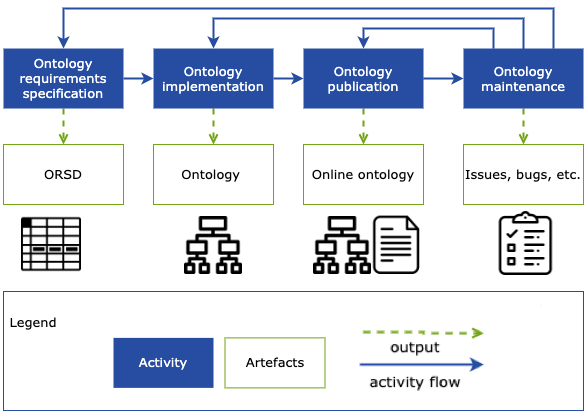
\includegraphics[width=0.6\linewidth]{figures/chp4-2_lot.png}
\caption[LOT Methodology]{Workflow proposed by the LOT Methodology~\parencite{poveda2022lot}.}
\label{fig:chp4-2_lot}
\end{figure}

\noindent\textbf{Maintenance}
Finally, the last stage of the development process, maintenance, refers to ontology updates as new requirements are found and/or errors are fixed. The ontology presented in this work promotes the gathering of issues or new requirements through the use of issues in the ontology GitHub repository. Additionally, it provides control of changes, and the documentation enables access to previous versions. Further details are shown in \cref{sec:chp4_pub-main}.



\subsection{Requirements}
\label{sec:chp4_requirements}
%\ana{añadir requisitos en anexo?}
This section presents the purpose, scope, and requirements of the Conceptual Mapping Ontology. In addition, it also describes from where and how the requirements are extracted: analysing the mapping languages (presented as a comparative framework in \cref{sec:chp4_framework}) and the Mapping Challenges proposed by the community.

\subsubsection{Purpose and scope}

The Conceptual Mapping ontology aims at gathering the expressiveness of declarative mapping languages that describe the transformation of heterogeneous data sources into RDF. This ontology-based language settles on the assumption that all mapping languages used for the same basic purpose of describing data sources in terms of an ontology to create RDF, must share some basic patterns and inherent characteristics. Inevitably, not all features are common. As described in previous sections, some languages were developed for specific purposes, others extend existing languages to cover additional use cases, and others are in turn based in languages that already provide them with certain capabilities. The Conceptual Mapping ontology is designed to represent and articulate these core features, which are extracted from two sources: (i) the analysis of current mapping languages, and (ii) the limitations of current languages identified by the community. These limitations, proposed by the W3C Knowledge Graph Construction Community Group\footnote{\label{foot:kgc}\url{https://www.w3.org/community/kg-construct/}}, are referred to as Mapping Challenges\footnote{\label{foot:challenges}\url{https://w3id.org/kg-construct/workshop/2021/challenges.html}} and have been partially implemented by some languages. %Both sources are described throughout this section.

This ontology also presents some limitations. As shown in \cref{sec:chp2_declarative_kgc}, mapping languages can be classified into three categories according to the schema in which they are based: RDF-based, SPARQL-based and based on other schemes. The Conceptual Mapping is included in the first category and, as such, has the same inherent capabilities and limitations as RDF-based languages regarding the representation of the language as an ontology. This implies that it is feasible to represent their expressiveness, whereas reusing classes and/or properties or creating equivalent constructs. Languages based on other approaches usually follow schemas that make them relatable to ontologies. This can be seen in the correspondence between YARRRML and RML: RML is written in Turtle syntax. YARRRML~\parencite{Heyvaert2018yarrrml} is mainly used as a user-friendly syntax to facilitate the writing of RML rules. It is based on YAML, and can easily be translated into RML\footnote{\url{https://rml.io/yarrrml/matey/}}. 

Lastly, SPARQL-based languages pose a challenge. SPARQL is a rich and powerful query language~\parencite{perez2009semantics} to which these mapping languages add more capabilities (e.g., SPARQL-Generate, SPARQL-Anything). It has an innate flexibility and capabilities sometimes not comparable to the other languages. For this reason, representing every single capability and feature of SPARQL-based languages is out of the scope of this work. Given the differences of representation paradigm between RDF and SPARQL for creating mappings, it cannot be ensured that the Conceptual Mapping covers all possibilities that a SPARQL-based language can, and as such, is considered a limitation.


\subsubsection{Mapping Challenges}
\label{sec:chp4_mapping_challenges}

Following its inception, the W3C Knowledge Graph Construction Community Group\cref{foot:kgc} defined a series of challenges for mapping languages based on the experience of members in using declarative mappings\cref{foot:challenges}. These challenges are a summary of the limitations of current languages. They have been partially addressed independently in some of the analyzed languages, such as RML~\parencite{delva2021rml-fields,iglesias2023rml} and ShExML~\parencite{garcia2021shexml-challenges}. These challenges are summarized as follows:

\begin{itemize}
    \item \textbf{[C1] Language Tags and Datatype.} It refers to dynamically building language tags [C1a] and datatypes [C1b], that is, from data rather than as constant values.
    \item \textbf{[C2] Iterators.} This challenge addresses the need to access data values 'outside' the iteration pattern [C2a], especially in \textcolor{black}{some tree-like data sources such as JSON}; and iterating over multi-value references [C2b].
    \item \textbf{[C3] Multi-value References.} It discusses how languages  handle data fields that contain multiple values [C3a], their datatypes and associated language tags [C3b].
    \item \textbf{[C4] RDF Collections and Containers.} This challenge addresses the need to handle RDF collections and containers.
    \item \textbf{[C5] Joins.} It refers to joining resources with zero join conditions [C5a] and joining literals instead of IRIs [C5b].
\end{itemize} 


\subsubsection{Conceptual Mapping Requirements}
\label{sec:chp4_cm-reqs}

In order to extract the requirements that serve as the basis for the development of the Conceptual Mapping ontology, we take as input the analysis from the comparison framework (\cref{sec:chp4_framework}) and the Mapping Challenges (\cref{sec:chp4_mapping_challenges}) described previously and the expertise of the authors. From a combination of their features, we extract 30 requirements. These requirements are expressed as facts, and are available in the ontology repository and portal\footnote{\url{https://oeg-upm.github.io/Conceptual-Mapping/requirements/requirements-core.html}}. Each requirement has a unique identifier, its provenance (comparison framework or mapping challenge id) and the corresponding constructs in the ontology. The constructs are written in Turtle, and lack cardinality restrictions for the sake of understandability. These requirements are tested with Themis, and its corresponding tests include these restrictions. More details on the evaluation of the requirements are provided in \cref{sec:chp4_cm-eval}. 

The requirements gathered range from general-purpose to fine-grained details. The general-purpose requirements refer to the basic fundamental capabilities of mappings, e.g., to create the rules to generate RDF triples (cm-r8) from reference data sources (cm-r7). The requirements with the next level of detail involve some specific restrictions and functionalities, e.g. to indicate the specific type (whether they are IRIs, Blank nodes, etc.) of subjects (cm-r16), predicates (cm-r17), objects (cm-r18), named graphs (cm-r19), datatypes (cm-r20) and language tags (cm-r21); the possibility of using linking conditions (cm-r23) and functions (cm-r15). Finally, some requirements refer to specific details or features regarding the description of data sources (e.g. cm-r4, cm-r6) and transformation rules (e.g. cm-r14, cm-r22, cm-r25).

Not all the observed features in the comparison framework have been added to the set of requirements. Some features are really specific, and supported by a minority of languages, sometimes only one language. As a result, we selected the (really) detailed features in these requirements to build the core specification of the Conceptual Mapping when they tackled the basic functionalities of the language. The rest of the details are left to be included as extensions. This differentiation and the modeling criteria is explained further in \cref{sec:chp4_implementation}.










\subsection{Implementation}
\label{sec:chp4_implementation}

This section describes in detail the activities and tasks carried out to implement the ontology, that consists in the conceptualization of the model, the encoding in a formal language, and the evaluation to fix errors, inconsistencies, and ensure that it meets the requirements. Additionally, an example of the ontology's use is presented at the end of the section.



\subsubsection{Ontology Conceptualization}




\begin{sidewaysfigure*}[]
    \centering
    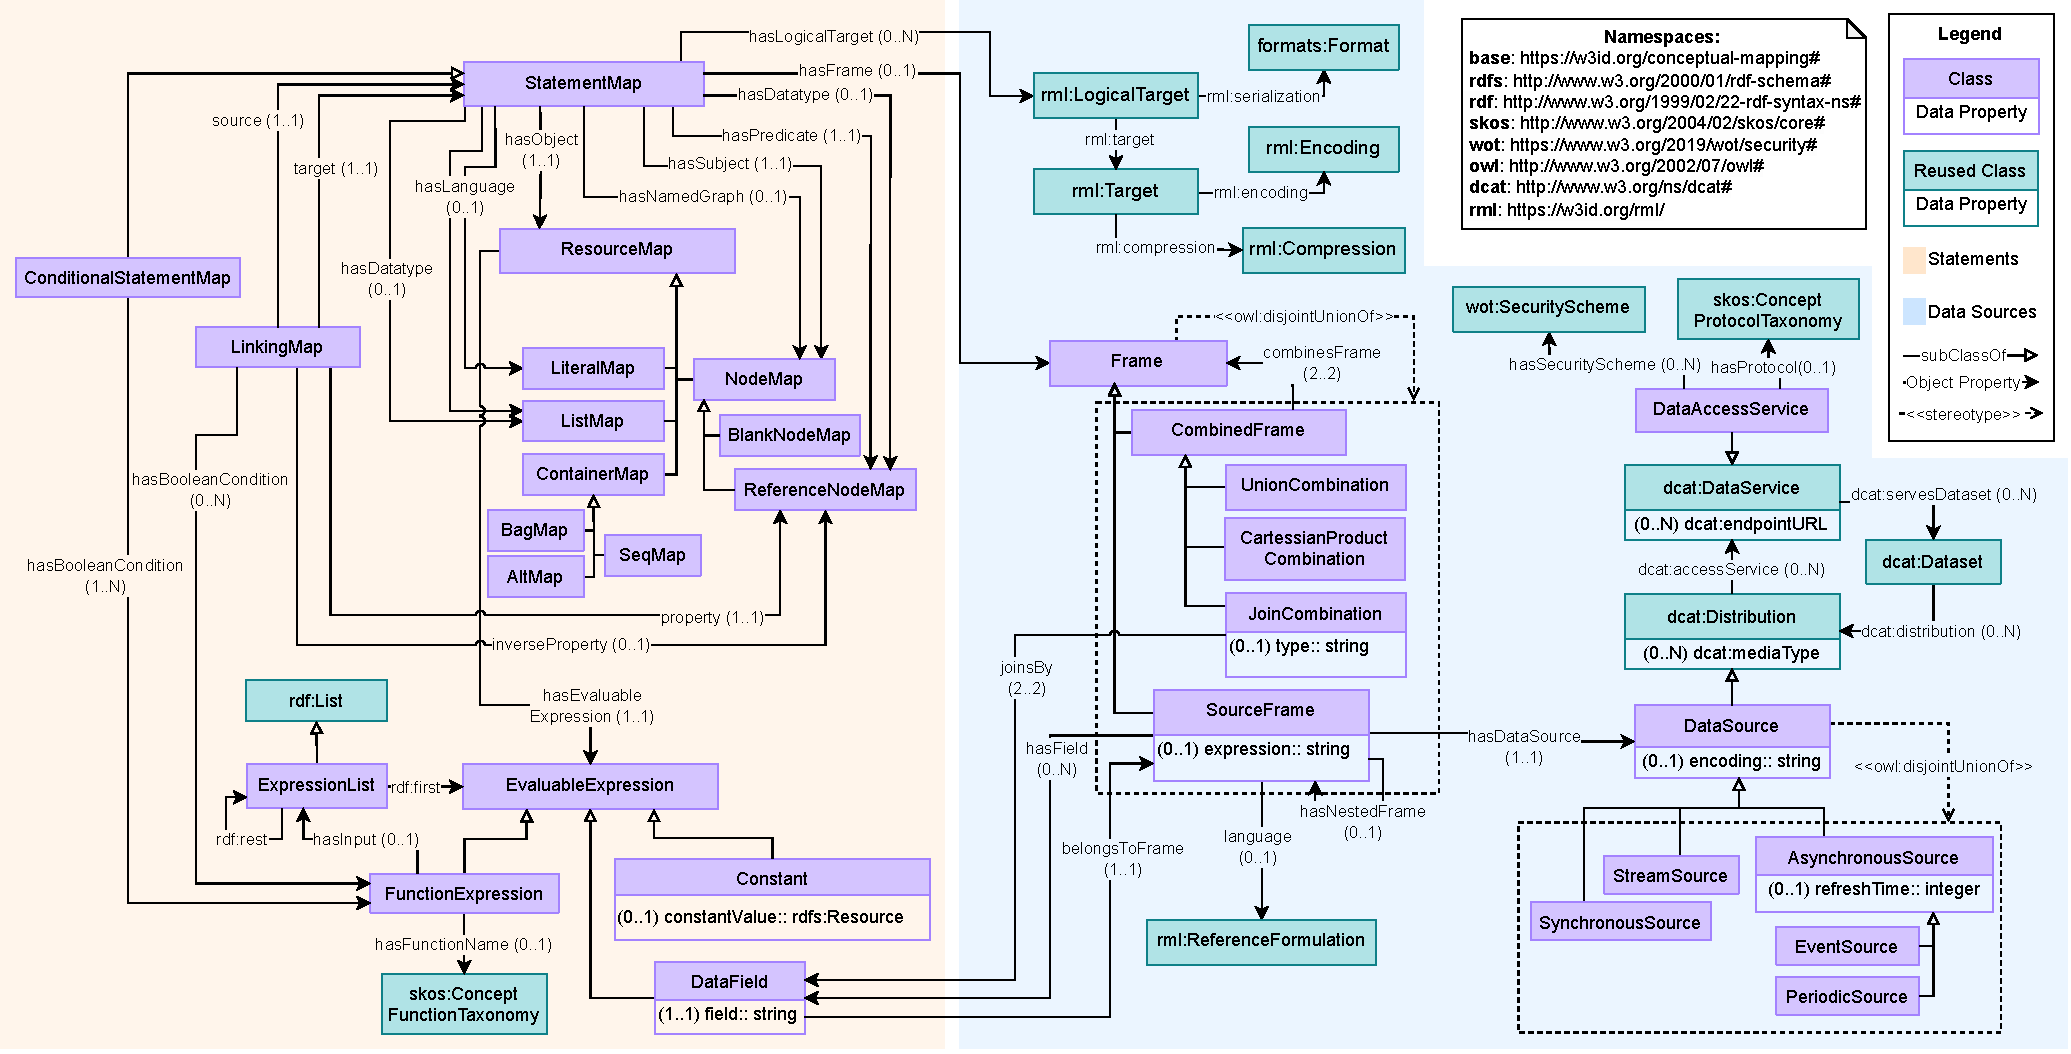
\includegraphics[width=1\linewidth]{figures/chp4-2_cm_diagram.pdf}
    \caption[Conceptual Mapping ontology overview]{Visual representation of the Conceptual Mapping ontology created using the Chowlk visual notation~\parencite{feria2022chowlk}.}
    \label{fig:chp4-2_cm_diagram}
\end{sidewaysfigure*}

\textcolor{black}{The ontology's conceptualization is built upon the requirements extracted from experts experience, a thorough analysis of the features and capabilities of current mapping languages presented as a comparative framework; and the languages' limitations discussed by the community and denoted as Mapping Challenges. The resulting ontology model is depicted in \cref{fig:chp4-2_cm_diagram}. This model represents the core specification of the Conceptual Mapping ontology that contains the essential features to cover the requirements. Some detailed features are also included when considered important to the language expressiveness, or needed for the language main functionality. Other detailed features are considered as extensions, as explained further in \cref{sec:chp4_cm-extensions}. For description purposes, we divide the ontology into two parts, \textit{Statements} and \textit{Data Sources}, that compose the core model. These two parts, when not used in combination, cannot describe a complete mapping. For that reason they are not separated into single modules. } 

\noindent\paragraph{\textbf{Data sources.}} A data source (\texttt{DataSource}) describes the source data that will be translated. For this section, the Data Catalog (DCAT) vocabulary~\parencite{albertoni2020dcat2} has been reused. \texttt{DataSource} is a subclass of \texttt{dcat:Distribution}, which is a specific representation of a dataset (\texttt{dcat:Dataset}), defined as ``data encoded in a certain structure such as lists, tables and databases''. A source can be a streaming source (\texttt{StreamSource}) that continuously generates data, a synchronous source (\texttt{SynchronousSource}) or an asynchronous source (\texttt{AsynchronousSource}). Asynchronous sources, in turn, can be event sources (\texttt{EventSource}) or periodic sources (\texttt{Periodic Source}). The details of the data source access are represented with the data access service class (\texttt{Data AccessService}), which in turn is a subclass of \texttt{dcat:DataService}. This class represents a collection of operations that provides access to one or more datasets or data processing functions, i.e., a description of how the data is accessed and retrieved. The data access service optionally has a security scheme (e.g., OAuth2, API Key, etc.) and an access protocol (e.g., HTTP(s), FTP, etc.).

Data properties in the \texttt{dcat:Dataset}, \texttt{dcat:Distribution} and \texttt{dcat:DataService} classes may be reused according to the features that may be represented in each mapping language, e.g. \texttt{dcat:endpointURL},  \texttt{dcat:accessURL} and \texttt{dcat:endpointDescrip\-tion}. A data access service is related to a security scheme. The class \texttt{wot:Securi\-tyScheme} (from the Web of Things (WoT) Security ontology\footnote{\label{foot:wotsec}\url{https://www.w3.org/2019/wot/security}}) has been reused. This class has different types of security schemes as subclasses and includes properties to specify the information on the scheme (e.g. the encryption algorithm, the format of the authentication information, the location of the authentication information). The security protocol \texttt{hasProtocol} has as set of predefined values that have been organized as a SKOS concept scheme. It contains almost 200 security protocols, e.g., HTTP(s), JDBC, FTP, GEO, among others. This SKOS list can be extended according to the users' needs by adding new concepts. 

In order to represent the fragments of data that are referenced in a statement map, the class \texttt{Frame} has been defined. They are connected with the property \texttt{hasFrame}. A frame can be a \texttt{SourceFrame} (base case) or a \texttt{CombinedFrame}, the latter representing two source frames or combined frames that are combined by means of a join (\texttt{JoinCombination}), a union (\texttt{UnionCombination}) or a cartessian product (\texttt{Cartessi\-anProductCombination}). 

A source frame corresponds to a data source (with \texttt{hasDataSource}) and defines which data is retrieved from the source and how it is fragmented (with \texttt{expression}). Among others, JSONPaths, XPaths, queries, or regular expressions can be expressed with this feature. \textcolor{black}{The language of the expression is defined with \texttt{language}, which domain is the reused class from RML \texttt{rml:ReferenceFormulation}}. A source frame may be related to another source frame with  \texttt{hasNest\-edFrame}, e.g. a frame is accessed firstly with a SPARQL query, and their results as a CSV file with this property. A source fragment may refer to many data fields (with \texttt{hasField}, which is the inverse property of \texttt{belongsToFrame}).

The desired output of the statements that are to be generated can be described with the imported \texttt{rml:LogicalTarget}, referenced by the optional property \texttt{hasLogicalTarget}. A \texttt{rml:LogicalTarget} specifies which RDF serialisation the output should be encoded (\texttt{rml:serialization}), and the referred \texttt{rml:Target}. 
The \texttt{rml:Target} indicates how the output target can be accessed,
and can describe: (i) the compression format for the RDF output (\texttt{rml:compression}) and, if so, how e.g., GZip,
and (ii) the encoding (\texttt{rml:encoding}), e.g., UTF-8.

\noindent\paragraph{\textbf{Statements.}} The central class of this section is the \texttt{StatementMap}, which represents a rule that defines for a triple its subject (\texttt{hasSubject}), predicate (\texttt{hasPredicate}), and object (\texttt{hasObject}). Optionally, it can also specify the object datatype (\texttt{hasDatatype}), language (\texttt{hasLanguage}) and assigned named graph (\texttt{hasNamedGraph}). Therefore, statement maps are similar to RDF statements as both of them are comprised by a subject, predicate and object. In statement maps, objects are resources (\texttt{ResourceMap}), and subjects and predicates are more specific, certain subclasses of the resource map: predicates are reference node maps (\texttt{ReferenceNodeMap}) that represent resources with an IRI, i.e., ontology properties. Subjects are node maps (\texttt{NodeMap}) that may be blank nodes (\texttt{Blank Node}) or also reference node maps. An object may be a literal (\texttt{LiteralMap}), a blank node, a container (\texttt{ContainerMap}) or a collection that defines a list (\texttt{ListMap}). The language is expressed as a literal, and the datatype is also a resource with an IRI, i.e. a reference node map.

Resource maps are expressed with an evaluable expression (\texttt{EvaluableExpression}) that may be a constant value (\texttt{Constant}), a function expression (\texttt{FunctionExpression}), or a data field (\texttt{DataField}) that belongs to some data source fragment (\texttt{belongsToFrame}). For function expressions, the function name (\texttt{hasFuntionName}) is taken from a set of predefined names organized in a SKOS concept scheme. This SKOS list can be extended according to the users' needs by adding new concepts for functions that have not been defined. Recursion in this function expression is represented through its input (\texttt{hasInput}) as an expression list (\texttt{ExpressionList}). Expression lists have been represented as a subclass of RDF lists (\texttt{rdf:List}), and the properties (\texttt{rdf:first}) and (\texttt{rdf:rest}) have been reused. Expression lists may have nested expression lists inside.


A special case of a statement map is a conditional statement map (\texttt{ConditionalSta\-tementMap}), a statement map that must satisfy a condition for the triples to be generated. The condition (\texttt{hasBooleanCondition}) is a function expression (e.g. if a value from a field called ``present'' is set to ``False'', the statement is not generated). Another relevant class is the linking map (\texttt{LinkingMap}), that enables linking subjects from a source (\texttt{source}) and a target (\texttt{target}) statement maps, i.e., two resources are linked and triples are generated if a linking condition is satisfied. Similarly to the conditional statement map, this condition is represented as a function expression.

\subsubsection{Ontology Design Patterns}
The following ontology design patterns \textcolor{black}{have been applied in the conceptualization as they are common solutions to the problem of representing taxonomies and linked lists}:
\begin{itemize}
    \item The SKOS vocabulary has been reused to represent some coding schemes such as the protocol taxonomy and the function taxonomy. \textcolor{black}{The design pattern consists on having an instance of} \texttt{skos:ConceptScheme} for each taxonomy, then each concept or term in the taxonomy, \texttt{skos:Concept}, is related to the corresponding concept scheme through the property \texttt{skos:inScheme}. The class that uses the taxonomy is then related to \texttt{skos:Concept} through an object property, e.g., class \texttt{DataAccessSer\-vice} and object property \texttt{hasProtocol}.
    \item The class \texttt{ExpressionList} uses the \textcolor{black}{design} pattern for lists developed in RDF where the properties \texttt{rdf:first} and \texttt{rdf:rest} are used to represent a linked list. The base case (first) is an evaluable expression whereas the rest of the list is (recursively)  an \texttt{ExpressionList}.
\end{itemize}

\subsubsection{Ontology evaluation}
\label{sec:chp4_cm-eval}


The ontology, implemented in OWL with Protégé, has been evaluated in different ways to ensure that it is correctly implemented, has no errors, inconsistencies or pitfalls, and meets the requirements.

\noindent\paragraph{\textbf{Reasoner.}} We used the reasoner Pellet in Protégé to look for inconsistencies in the model, and the results showed no errors.

\noindent\paragraph{\textbf{OOPS!.}}~\parencite{poveda2014oops} This tool was used to identify modeling pitfalls in the ontology. We executed the tool several times to fix the pitfalls, until there were no important ones. Currently, the results of OOPS! show pitfalls from the reused ontologies, but none important for the newly created terms and axioms. One minor pitfall is returned, P13, regarding the lack of inverse relationships, which we consider that are not  needed in the ontology. The rest of the pitfalls are as follows: P08 (missing annotations) from DCTERMS; P11 (missing domain or range in properties) for DCTERMS, DCAT and SKOS; and P20 (missing ontology annotations) for DCAT.

\noindent\paragraph{\textbf{Themis.}}~\parencite{fernandez2021themis} Themis is a tool able to evaluate whether the requirements are implemented in the ontology. To that end, the requirements must be provided in a specific syntax or described with the Verification Test Case (VTC) ontology\footnote{\url{https://albaizq.github.io/test-verification-ontology/OnToology/ontology/verification-test-description.ttl/documentation/index-en.html}}. The requirements of the Conceptual Mapping were translated to create the corresponding tests, and were tested in the tool with success. The requirements and associated test along with the complete set of tests annotated with the VTC ontology are available in the GitHub repository\footnote{\url{https://github.com/oeg-upm/Conceptual-Mapping/tree/main/requirements}}.

\noindent\paragraph{\textbf{FOOPS!.}}~\parencite{garijo2021foops} Additionally, we tried running FOOPS! to check the FAIRness of the ontology, resulting in 73\%, which is acceptable. To improve the score, the ontology should be added to a registry and have more metadata describing it, and use a persistent base IRI. 

With these evaluations, we can conclude that the ontology is correctly encoded and implemented, and that it meets the requirements specified in \cref{sec:chp4_requirements}. 



\subsection{Publication and Maintenance}
\label{sec:chp4_pub-main}

In order to publish the ontology, the first step required is to create the ontology documentation. We used Widoco~\parencite{garijo2017widoco}, integrated inside the OnToology~\parencite{alobaid2019automating} system, to automatically generate and update the HTML documentation every time there is a commit in the GitHub repository where the ontology is stored. This documentation contains the ontology metadata, links to the previous version, a description of the ontology, the diagram, and detailed examples of the capabilities of the language. It is published using a W3ID URL\cref{foot:cmlink} and under the CC BY-SA 4.0 license.

The HTML documentation is not the only documentation resource provided. An overview of all resources is provided in the ontology portal\cref{foot:cmportal}. This portal shows in a table the ontologies associated with the Conceptual Mapping ontology. For now, the core (Conceptual Mapping) and an extension to describe CSV files in detail (Conceptual Mapping - CSV Description) are available. For each ontology, links to the HTML documentation, the requirements, the GitHub repository, the Issue Tracker, and the releases are provided. 

The maintenance is supported by the Issue Tracker\footnote{\url{https://github.com/oeg-upm/Conceptual-Mapping/issues}}, where proposals for new requirements, additions, deletions or modifications can be added as GitHub issues. This approach allows authors to review the proposals and discuss their possible implementation.



\subsection{Extensions}
\label{sec:chp4_cm-extensions}
The Conceptual Mapping ontology has been designed as a core ontology. However, as time passes, new requirements may emerge. In order to include these new requirements, new modules of the Conceptual Mapping ontology shall be developed. It is worth mentioning that this is a common practice for ontologies, which is highly suitable for adapting an existing ontology to new scenarios, by ontology modules specialized for a specific set of requirements. A clear example of this is the SAREF ontology\footnote{\url{https://saref.etsi.org/}}, that has a core module\footnote{\url{https://saref.etsi.org/core/v3.1.1/}} and then specific extensions\footnote{\url{https://saref.etsi.org/extensions.html}} for certain domains, such as energy (SAREF4ENER) or buildings (SAREF4BLDG) among others. For the Conceptual Mapping we present two extensions: for allowing a more detailed description of CSV files, and for generating RDF-star graphs.


\begin{figure}[!t]
\centering
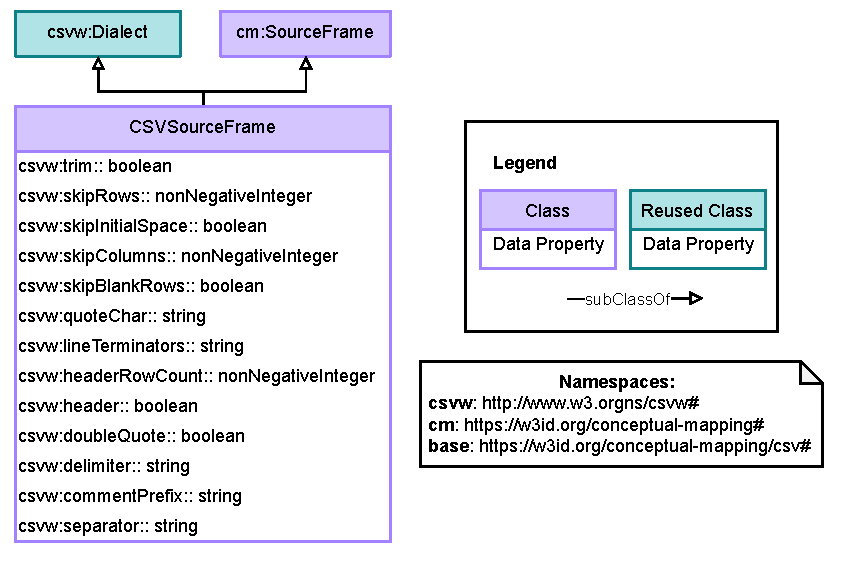
\includegraphics[width=0.8\linewidth]{figures/chp4-2_cm-csv.pdf}
\caption[CM-CSV module]{Conceptualization of the CM-CSV module following the Chowlk visual notation~\parencite{feria2022chowlk}.}
\label{fig:chp4-2_cm-csv}
\end{figure}


\subsubsection{CSV description: CM-CSV}
The core module of the Conceptual Mapping includes limited possibilities for describing CSV files in depth. The extension CM-CSV\footnote{\url{https://w3id.org/conceptual-mapping/csv}} provides extended features to this end. Thus, the CSVW~\parencite{Tennison2015csvw} proposal has been blended as an ontology module linked to the core Conceptual Mapping ontology. The class \texttt{CSVSourceFrame} is created as a subclass of \texttt{SourceFrame} and \texttt{csvw:Dialect} to inherit their characteristics. This module is depicted in \cref{fig:chp4-2_cm-csv}. Thus, this extension allows to describe CSV characteristics such as if the file contains headers (\texttt{csvw:header}), its delimiter (\texttt{csvw:delimiter}), separator (\texttt{csvw:separator}), among many others. 

\subsubsection{RDF-star generation: CM-star}
\label{sec:chp4_cm-star}
RDF-star~\parencite{hartig2017foundations} was recently proposed as a compact alternative for reification in RDF. It extends the RDF syntax introducing the notion of \textit{Quoted triples}, i.e. triples that can be placed in the position of objects and/or subjects. These triples can be inserted in the graph outside the quoted triple (i.e. they are \textit{asserted}), or appear only inside another triples (i.e. they are \textit{non-asserted}).

RDF-star has quickly gained popularity, leading
to its adoption by a wide range of systems~\footnote{\url{https://w3c.github.io/rdf-star/implementations.html}} (e.g., Apache Jena~\footnote{\url{https://jena.apache.org}}, Oxigraph~\parencite{oxigraph}) and the formation of the RDF-star Working Group\footnote{\url{https://www.w3.org/groups/wg/rdf-star}}. 
Regarding mapping languages, SPARQL-Anything is able to generate RDF-graphs as it natively implements the updates from Apache Jena; RML was extended for this purpose with the RML-star module~\parencite{iglesias2022rmlstar,delva2021rml-star,iglesias2023rml} (explained in detail in \cref{sec:chp4_rml_star}), as well as R2RML-star~\parencite{sundqvist2022extending}.

\begin{figure}[!t]
\centering
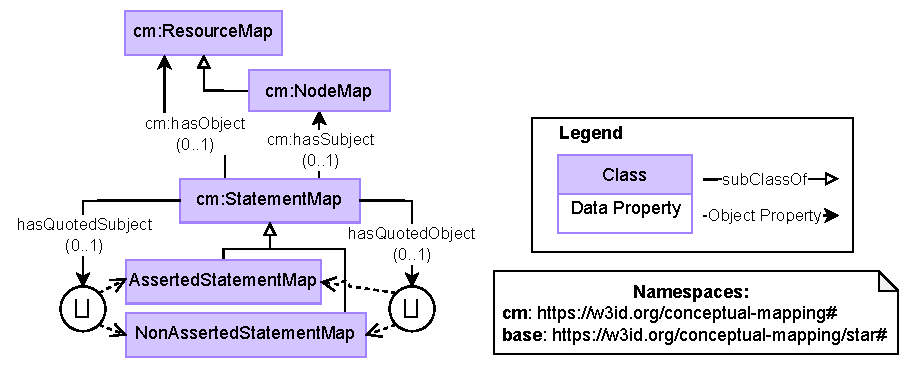
\includegraphics[width=0.9\linewidth]{figures/chp4-2_cm-star.pdf}
\caption[CM-star module]{Conceptualization of the CM-star module following the Chowlk visual notation~\parencite{feria2022chowlk}.}
\label{fig:chp4-2_cm-star}
\end{figure}




As a result, we developed a module to cover this new feature. The Conceptual Mapping implements the RDF-star graph generation adopting the recursive nature of quoted triples in the CM-star module\footnote{\url{https://w3id.org/conceptual-mapping/star}}. \cref{fig:chp4-2_cm-star} represents the overview of this module. Two subclasses of \texttt{StatementMap} are created to denote asserted (\texttt{AssertedStatementMap}) and non-asserted (\texttt{NonAssertedStatementMap}) statement maps. These statements can be quoted as subjects and objects with the properties \texttt{hasQuotedSubject} and \texttt{hasQuotedObject} respectively. The range of these properties is the union of the introduced statement subclasses. This extension enables potentially an infinite number of quoted statements, as the RDF-star specification indicates~\parencite{hartig2023rdf}. 



\subsection{Ontology usage example}\label{sec:cm_example} 



\begin{figure}[t!]
    \centering
    \begin{subfigure}[b]{0.45\linewidth}
        \centering
    	\includegraphics[width=1\linewidth]{figures/chp4-2_example_ont}
    	\caption{Example reference ontology that represents the classes \texttt{City} and \texttt{Location}, linked by the property \texttt{eg:location}.}
    	\label{fig:chp4-2_chp4_ex_onto}
    \end{subfigure}
    \begin{subfigure}[b]{0.28\linewidth}
        \centering
    	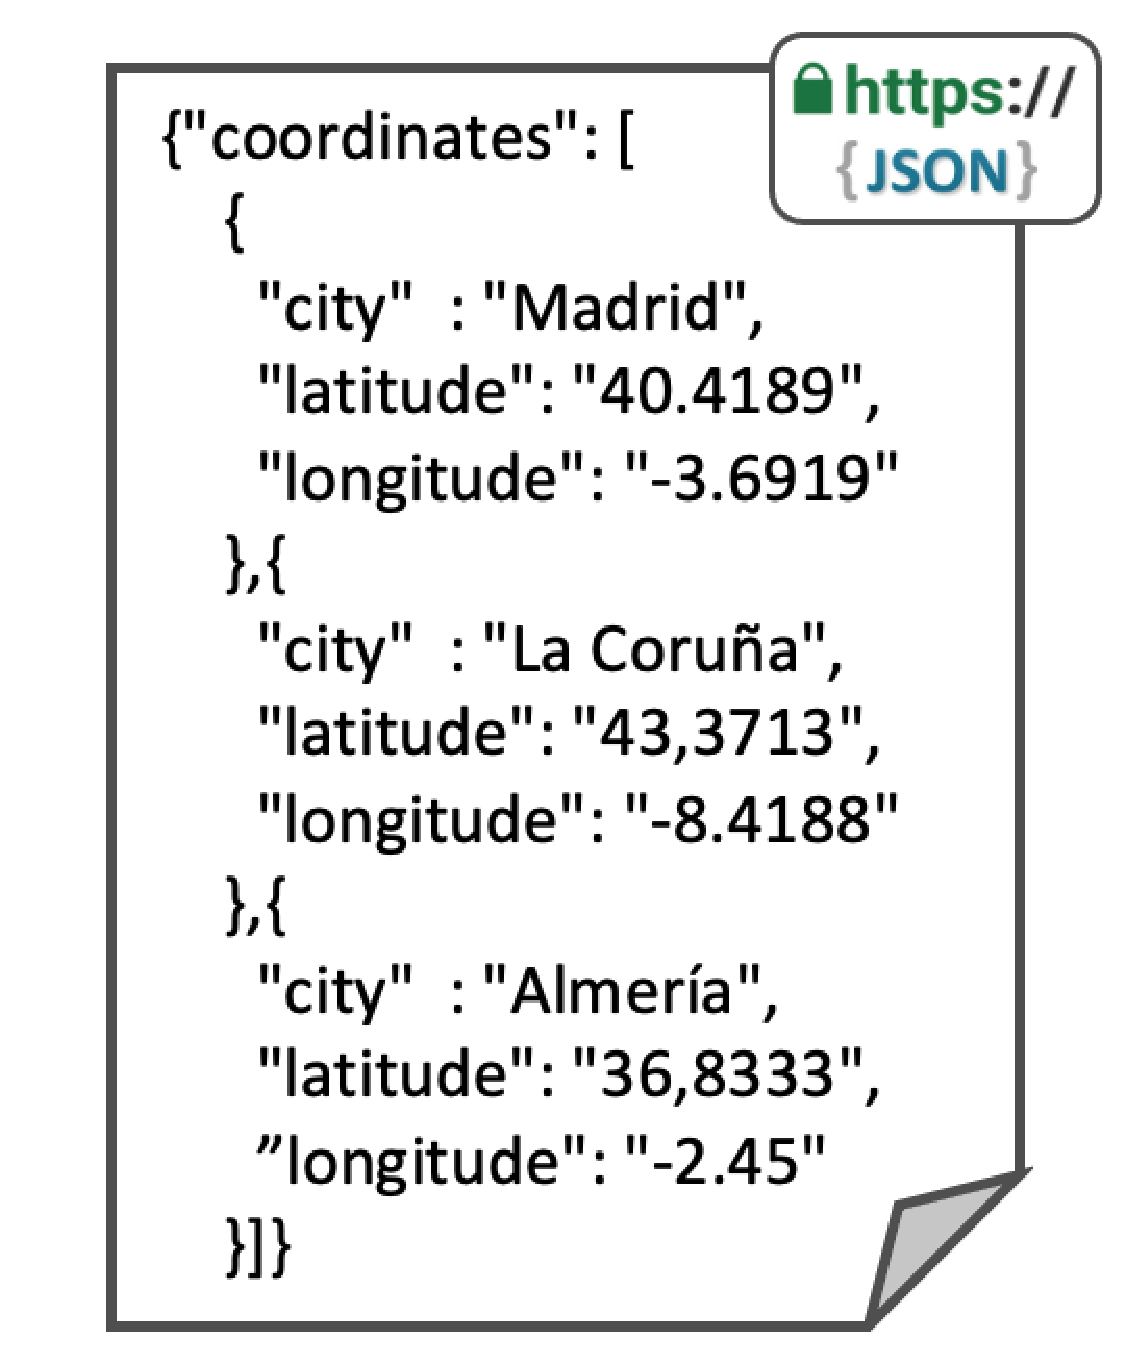
\includegraphics[width=1\linewidth]{figures/chp4-2_example_json}
    	\caption{Example input JSON file ```coordinates.json".}
    	\label{fig:chp4-2_chp4_ex_json}
    \end{subfigure}
    \begin{subfigure}[b]{0.7\linewidth}
        \centering
    	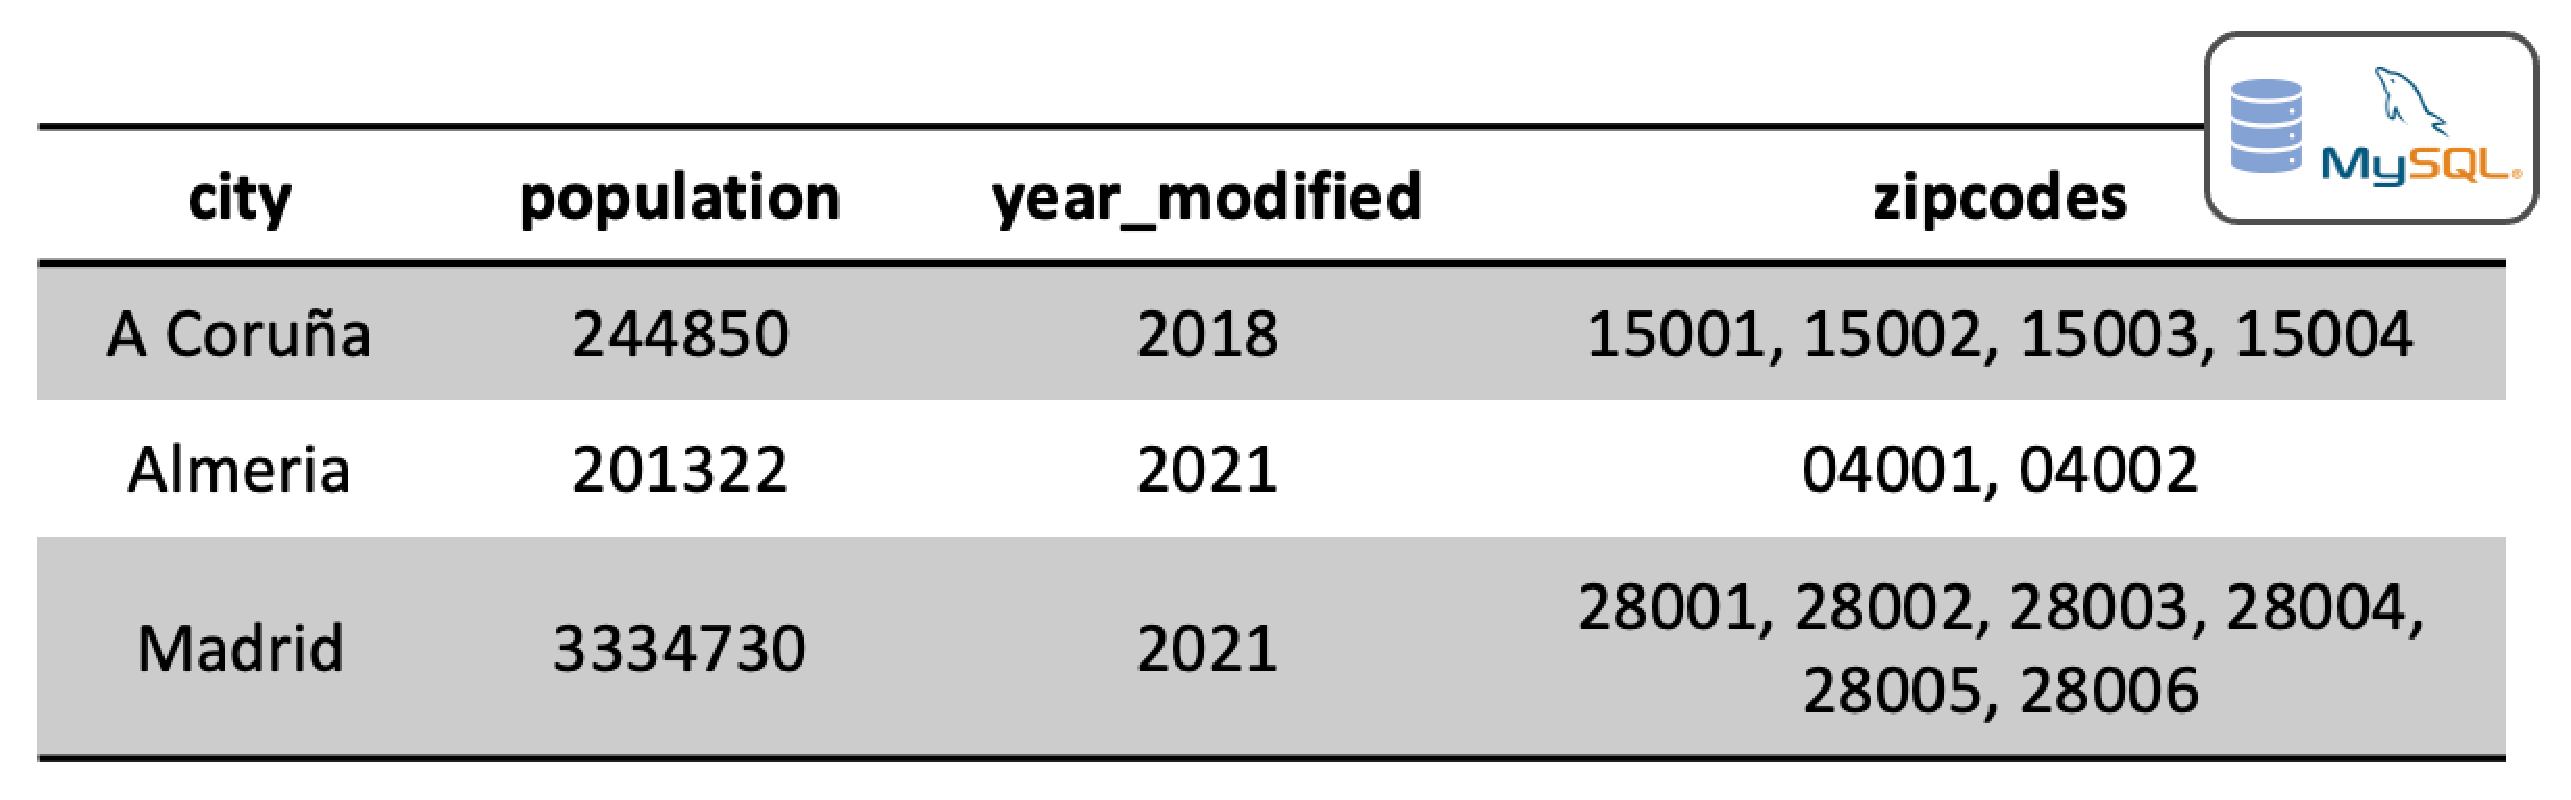
\includegraphics[width=1\linewidth]{figures/chp4-2_example_rdb}
    	\caption{Example input MySQL table ```cities".}
    	\label{fig:chp4-2_chp4_ex_rdb}
    \end{subfigure}
    \caption[Example data and ontology about cities for CM mapping]{Input source data and reference ontology that represents information on cities and their location.}
    \label{fig:chp4-2_chp4_ex_input}
\end{figure}



%\ana{no sé si dejar esto o rehacer y poner de drugs4covid, para que no sean datos de juguete. O si acaso poner que sea un use case, eso requeriría de hacer el mapping también en otros lenguajes. Por ahora dejar como está}

This section builds a mapping in three steps (data sources in \cref{lst:chp4_cm_sources}, triples in \cref{lst:chp4_cm_spo} and special statements in \cref{lst:chp4_cm_general}) to represent how the proposed language can describe data with different features. The mapping uses the data sources ``coordinates.json" (\cref{fig:chp4-2_chp4_ex_json}) and ``cities" (\cref{fig:chp4-2_chp4_ex_rdb}) as input and the ontology depicted in  \cref{fig:chp4-2_chp4_ex_onto} as reference, to create the output RDF shown in \cref{lst:chp4_output}. 
%Additionally, \cref{appendix2}\ana{APENDIX!!} contains a second example to illustrate different features than the ones represented in the example of this section, to provide more insights about the expressiveness of this language.

\begin{captionedlisting}{lst:chp4_output}{Expected RDF output for the data sources and the ontology in \cref{fig:chp4-2_chp4_ex_input}.}
\centering
{\begin{lstlisting}[]
<http://ex.com/loc/40.4189--3.6919> a eg:Location ;
	eg:lat "40.4189"^^xsd:decimal ;
	eg:long "-3.6919"^^xsd:decimal .
<http://ex.com/loc/43.3713--8.4188> a eg:Location ;
	eg:lat "43.3713"^^xsd:decimal ;
	eg:long "-8.4188"^^xsd:decimal .
<http://ex.com/loc/36.8333--2.45> a eg:Location ;
	eg:lat "36.8333"^^xsd:decimal ;
	eg:long "-2.45"^^xsd:decimal .
<http://ex.com/city/ACoruña> a eg:City ;
	eg:zipcode 15001, 15002, 15003, 15004 ;
	eg:location <http://ex.com/loc/43.3713--8.4188> .
<http://ex.com/city/Almería> a eg:City ;
	eg:zipcode 04001, 04002 ;
	eg:population 201322 ;
	eg:location <http://ex.com/loc/36.8333--2.45> .
<http://ex.com/city/Madrid> a eg:City ;
	eg:zipcode 28001, 28002, 28003, 28004, 28005, 28006;
	eg:population 3334730 ;
	eg:location <http://ex.com/loc/40.4189--3.6919> .
\end{lstlisting}}
\end{captionedlisting}

\noindent\paragraph{\textbf{Data sources.}} \cref{lst:chp4_cm_sources} shows the description of the json file ``coordinates.json" indicating the protocol from the SKOS concept scheme (\texttt{cmp:https}), media type (``application/json"), JSONPath to extract data, access URL  ``https://ex.com/geodata/coordi\-nates.json", and  fields that are going to be used in the transformation. There is no security scheme. The MySQL table ``cities" also has no security scheme, the protocol needed is \texttt{cmp:jdbc}, the database access is specified in the endpoint URL, and the table as an SQL query. The fields are also specified, with the special case of ``zipcodes" that needs a \texttt{cm:hasNestedFrame} to extract multiple values inside the field.

\begin{captionedlisting}{lst:chp4_cm_sources}{Description with the Conceptual Mapping of two data sources (a JSON file and a relational database), their access and fields.}
\centering
{\begin{lstlisting}[language=concm,firstnumber=1]
# Locations
:FrameLoc a cm:SourceFrame;
  cm:expression "$\dollar$.coordinates[*]";
  cm:language ql:JSONPath ;
  cm:hasField :lat;
  cm:hasField :long;
  cm:hasField :loc_city;
  cm:hasDataSource [ a cm:SynchronousSource;
    dcat:mediaType "text/json";
    dcat:accessService [
      cm:hasProtocol cmp:https;
      dcat:endpointURL "https://ex.com/geodata/coordinates.json" 
      cm:hasSecurityScheme [ a wotsec:NoSecurityScheme; ];
    ] ;
  ] .

:lat a cm:DataField ; cm:field "$\dollar$.latitude" .
:long a cm:DataField ; cm:field "$\dollar$.longitude" .
:loc_city a cm:DataField; cm:field "$\dollar$.city" .

# Cities
:FrameCities a cm:SourceFrame ;
  cm:expression "SELECT * FROM cities;";
  cm:hasField :c_city;
  cm:hasField :population;
  cm:hasField :year;
  cm:hasNestedFrame [
    cm:expression "$\dollar$.zipcodes[*]";
    cm:hasField :zipcode ];
  cm:hasDataSource [ a cm:SynchronousSource;
    dcat:mediaType "text/plain";
    dcat:accessService [
      cm:hasProtocol cmp:jdbc;
      dcat:endpointURL "jdbc:mysql://localhost:3306/citydb";
      cm:hasSecurityScheme [a wotsec:NoSecurityScheme;] ].

:c_city a cm:DataField; cm:field "city" .
:population a cm:DataField; cm:field "population" .
:year a cm:DataField; cm:field "year_modified" .
:zipcode a cm:DataField cm:field "zipcodes" .
\end{lstlisting}}
\end{captionedlisting}

%\noindent{\textbf{Locations.}} Sarah is working at the National Geographic Institute from Spain, and manages everyday information about places and locations. She wants to create a knowledge graph with the geographical data that she usually manages. She starts writing a mapping (\cref{lst:uc1}) to represent cities from a local JSON file, \texttt{Venue.json} (\cref{lst:data_venues}). This data will be transformed into instances of the class \texttt{City}. 

\noindent\paragraph{\textbf{Statements.}} \cref{lst:chp4_cm_spo} contains the rules needed to create instances of the classes \texttt{eg:Location} and \texttt{eg:City}; and their following attributes: \texttt{eg:lat} and \texttt{eg:long} for the former; \texttt{eg:zipcode} for the latter. To correctly generate the URI for the instances of \texttt{eg:City}, a replace function inside a concatenate function is needed to (1) remove the blank spaces in the field ``city" and (2) add the field to the base URI ``http://ex.com/city/".

\begin{captionedlisting}{lst:chp4_cm_spo}{Description with the Conceptual Mapping of the creation of regular statements from the data sources described in \cref{lst:chp4_cm_sources}.}
\centering
{\begin{lstlisting}[language=concm,firstnumber=1]
# Locations
:SubjectLoc a cm:ReferenceNodeMap ;
  cm:hasEvaluableExpression [
    cm:hasFunctionName cmf:concat; 
    cm:hasInput ([cm:constantValue "http://ex.com/loc/"]    :lat [cm:constantValue "-" ] :long)].

:StatementLoc1 a cm:StatementMap ;
  cm:hasFrame :FrameLoc ;
  cm:subject :SubjectLoc ;
  cm:predicate [ a cm:ReferenceNodeMap; 
    cm:hasEvaluableExpression [cm:constantValue rdf:type ] ];
  cm:object [cm:hasEvaluableExpression [cm:constantValue eg:Location]].

:StatementLoc2 a cm:StatementMap ;
  cm:hasFrame :FrameLoc ;
  cm:subject :SubjectLoc ;
  cm:predicate [ a cm:ReferenceNodeMap; 
    cm:hasEvaluableExpression [cm:constantValue eg:lat]];
  cm:object [ a cm:Literal; cm:hasEvaluableExpression :lat];
  cm:hasDatatype [cm:hasEvaluableExpression xsd:decimal].

:StatementLoc3 a cm:StatementMap ;
  cm:hasFrame :FrameLoc ;
  cm:subject :SubjectLoc ;
  cm:predicate [ a cm:ReferenceNodeMap; 
    cm:hasEvaluableExpression [cm:constantValue eg:long]];
  cm:object [ a cm:Literal; cm:hasEvaluableExpression :long];
  cm:hasDatatype [ cm:hasEvaluableExpression xsd:decimal].
    
# Cities
:city_ns a cm:FunctionExpression ;
  cm:functionName cmf:replace ;
  cm:hasInput (c_city " " "")

:SubjectCities a cm:ReferenceNodeMap;
  cm:hasEvaluableExpression [
    cm:hasFunctionName cmf:concat; 
    cm:hasInput ([cm:constantValue "http://ex.com/city/"] :city_ns)].

:StatementCit1 a cm:StatementMap ;
  cm:hasFrame :FrameCities ;
  cm:subject :SubjectCities ;
  cm:predicate [ a cm:ReferenceNodeMap; 
    cm:hasEvaluableExpression [cm:constantValue rdf:type]];
  cm:object [ a cm:ReferenceNodeMap; 
    cm:hasEvaluableExpression  [cm:constantValue eg:City]] .

:StatementCit2 a cm:StatementMap ;
  cm:hasFrame :FrameCities ;
  cm:subject :SubjectCities ;
  cm:predicate [ a cm:ReferenceNodeMap; 
    cm:hasEvaluableExpression [cm:constantValue rdfs:label]];
  cm:object [ a cm:ReferenceNodeMap; 
    cm:hasEvaluableExpression  [cm:constantValue :c_city]] .
  cm:hasLanguage [ cm:hasEvaluableExpression [ cm:constantValue "es" ] ].

:StatementCit3 a cm:StatementMap ;
  cm:hasFrame :FrameCities ;
  cm:subject :SubjectCities ;
  cm:predicate [ a cm:ReferenceNodeMap; 
    cm:hasEvaluableExpression [cm:constantValue eg:zipcode] ];
  cm:object [ a cm:Literal;
    cm:hasEvaluableExpression [cm:constantValue :zipcode] ];
  cm:hasDatatype [ cm:hasEvaluableExpression xsd:integer ].
\end{lstlisting}}
\end{captionedlisting}


\noindent\paragraph{\textbf{Special statements.}} \cref{lst:chp4_cm_general} describes how a conditional statement and a linking rule are generated. This description is represented by means of functions. With the property \texttt{cm:hasBooleanCondition}, the conditional statement declares that the field \texttt{:year} has to be greater than 2020. The linking rule performs the link between the instances of \texttt{eg:City} and \texttt{eg:Location} with the predicate \texttt{eg:location}, using a distance metric (levenshtein function) that has to be greater then a threshold of ``0.75". 

\begin{captionedlisting}{lst:chp4_cm_general}{Conditional and linking rules described with the Conceptual Mapping that complement the data source description and regular statements described in \cref{lst:chp4_cm_sources} and \cref{lst:chp4_cm_spo}.}
\centering
{\begin{lstlisting}[language=concm,firstnumber=1]
:StatementCit4 a cm:ConditionalStatementMap ;
  cm:hasFrame :FrameCities ;
  cm:subject :SubjectCities ;
  cm:predicate [ a cm:ReferenceNodeMap; 
    cm:hasEvaluableExpression [cm:constantValue eg:population] ];
  cm:object [ a cm:Literal; 
    cm:hasEvaluableExpression  [cm:constantValue :population] ];
  cm:hasDatatype [ cm:hasEvaluableExpression xsd:integer];
  cm:hasBooleanCondition [
    cm:functionName cmf:greater_than ;
    cm:hasInput ( :year 2020 ) ] .

:LinkExp1 a cm:LinkingExpression ;
  cm:source :StatementCit1 ;
  cm:target :StatementLoc1 ;
  cm:property eg:location ;
  cm:hasBooleanCondition [
    cm:functionName cmf:greater_than ; 
    cm:hasInput ( :levfun 0.75 ) ] .

:levfun a cm:FunctionExpression ;
  cm:functionName cmf:levenshtein_distance ;    
  cm:hasInput (:c_city :loc_city) .
\end{lstlisting}}
\end{captionedlisting}









\section{Mapping Rules for RDF-star: RML-star}
\label{sec:chp4_rml_star}

%In the late years, the RDF-star~(\cite{hartig2017foundations}) approach for reification has gained popularity. Along with its expansions, different semantic web technologies have been updated to include this new syntax\footnote{\url{https://w3c.github.io/rdf-star/implementations}}. This section describes one of these updates related to building RDF-star graphs: RML-star. \ana{esto no liga del todo bien con lo anterior}



Making statements about statements in RDF has
posed a challenge almost since the inception of RDF.
The W3C RDF Primer~(\cite{manola2004rdf}) already included a description of the standard reification approach to tackle this issue.
Other alternatives were proposed over the years,
such as named graphs~(\cite{carroll2005namedgraphs}), N-ary relationships~(\cite{naryw3c2006}), singleton properties~(\cite{nguyen2014don}), RDF$^+$~(\cite{schueler2008querying}), and more recently, \mbox{RDF-star}~(\cite{hartig2017foundations}). 

RDF-star does not leverage the characteristics of RDF as the others proposals. Instead it extends the RDF syntax to introduce the notion of \texttt{embedded triples}. This approach is currently under development to become a W3C standard\footnote{\url{https://www.w3.org/groups/wg/rdf-star}}. 
As a consequence, an increasing number of semantic technologies are supporting this proposal\footnote{\url{https://w3c.github.io/rdf-star/implementations}}, which include triplestores (e.g. GraphDB, AnzoGraph) and programming libraries (e.g. Apache Jena, Oxigraph).

It is possible to construct reified RDF graphs using mappings with the reification approaches abovementioned, except for RDF-star. As this proposal extends the original RDF syntax, it requires mapping languages to adapt and evolve in order to construct RDF-star graphs. This chapter presents the extension of the RML language to enable the construction of RDF-star graphs, RML-star. We first introduce how reified RDF graphs can be constructed using RML with different reification approaches, and then we present RML-star. This proposal is validated with \mbox{Morph-KGC$^{star}$}, a KG construction engine that implements our proposal.

%This section describes popular reification approaches and shows how they can be used in RML and RML-star with a running example. 
%Standard reification and singleton properties are considered in Section \ref{sec:chp4_validation}, showing that \mbox{Morph-KGC$^{star}$} does not add any overhead in the time required to generate the \mbox{RDF-star} triples compared to them.

\subsection{Statements about statements in mapping rules}
\label{sec:chp4_reif_mappings}

We illustrate each reification alternative presented throughout this section with a running example that uses the data shown in \cref{lst:chp4_csv_star}.
It contains CSV data related to pole vault:
the vaulter (\texttt{PERSON}),
the height of the jump (\texttt{MARK}),
the date when the jump was performed (\texttt{DATE}) and
an identifier of the jump (\texttt{ID}).
The running example represents
that a person jumped some height on a specific date, i.e., it adds the metadata about ``date''
to the statement ``a person jumped some height''.

\noindent\hspace{0.15\linewidth}\begin{minipage}{\linewidth}
\begin{captionedlisting}{lst:chp4_csv_star}{Contents of the logical source \texttt{:marks} in CSV format.}
\centering
\begin{tabular}{c}
\hspace{3em}
{\begin{lstlisting}[basicstyle=\ttfamily\small,label={list:example1},columns=flexible]
ID  , DATE       , MARK ,   PERSON
1   , 2022-03-21 , 4.80 ,   Angelica
2   , 2022-03-19 , 4.85 ,   Katerina
\end{lstlisting}}
\end{tabular}
\end{captionedlisting}
\end{minipage}

\subsubsection{Reification with RML}

There are several reification approaches for RDF as presented in \cref{chp2_reification}, such as standard reification, singleton properties, N-ary relationships or named graphs. 
These approaches use strategies that add metadata to triples
without modifying the original RDF syntax.
Thus, they can be used with RML without any further modification. RML mapping rules enable the generation of blank nodes (required for the standard reification approach), dynamically generated predicates (required for the singleton properties approach) and named graphs (required for the named graphs approach). %\ana{si voy con todos, influye en el ejemplo de aquí abajo y en los use cases. En ese caso, quitar somef (demasiado grande el mapping, con semmeddb es suficiente)}

%\ana{probablemente en sota estarán explicados cada uno de los modelos, probablemente no haga falta ponerlos aquí también.}


\noindent\textbf{\textit{Standard Reification}}~(\cite{manola2004rdf}) was proposed in the W3C RDF Primer~(\cite{manola2004rdf}).
It assigns statements to unique identifiers (typically blank nodes) typed with \texttt{rdf:Statement} and described using the properties \texttt{rdf:subject}, \texttt{rdf:predicate} and \texttt{rdf:object}.
This way, the unique identifier representing the statement can be further annotated with additional statements. \cref{lst:chp4_res-std-reif} shows an example of standard reification for the data in \cref{lst:chp4_csv_star}, created with the RML mapping rules in \cref{lst:chp4_std-reif}. 
This mapping creates blank nodes in the subject with the \texttt{ID} data field, typed with \texttt{rdf:Statement}; and has three predicate object maps to generate the \texttt{rdf:subject}, \texttt{rdf:predicate}, \texttt{rdf:object} of the triples (\textit{An athlete jumps certain height}) and a predicate object map to annotate the statements with \texttt{:date} (\textit{in a specific date}).




\begin{minipage}{\linewidth}
\begin{captionedlisting}{lst:chp4_std-reif}{Example RML mapping using standard reification that transforms data in \cref{lst:chp4_csv_star}.}
\centering
\begin{multicols}{2}
{\begin{lstlisting}[basicstyle=\ttfamily\small,label={list:example1},columns=flexible]
<#TM> a rr:TriplesMap ;
  rml:logicalSource :marks ;
  rr:subjectMap [ 
    rml:reference "ID" ;
    rr:termType rr:BlankNode ;
    rr:class rdf:Statement  ] ;
  rr:predicateObjectMap [ 
    rr:predicate rdf:subject ;
    rr:objectMap [
      rr:template ":{PERSON}" ] ] ;
  rr:predicateObjectMap [ 
    rr:predicate rdf:predicate ;
    rr:object :jumps ] ;
  rr:predicateObjectMap [ 
    rr:predicate rdf:object ;
    rr:objectMap [
      rml:reference "MARK" ] ] ;
  rr:predicateObjectMap [ 
    rr:predicate :date ;
    rr:objectMap [
      rml:reference "DATE" ] ] .
\end{lstlisting}}
\end{multicols}
\end{captionedlisting}
\end{minipage}

\begin{minipage}{\linewidth}
\begin{captionedlisting}{lst:chp4_res-std-reif}{RDF triples generated by the mapping in \cref{lst:chp4_std-reif}.}
\centering
\begin{multicols}{2}
{\begin{lstlisting}[basicstyle=\ttfamily\small,label={list:example1},columns=flexible]
_:1 rdf:type      rdf:Statement .
_:1 rdf:subject   :Angelica .
_:1 rdf:predicate :jumps .
_:1 rdf:object    "4.80" .
_:1 :date         "2022-03-21" .
_:2 rdf:type      rdf:Statement .
_:2 rdf:subject   :Katerina .
_:2 rdf:predicate :jumps .
_:2 rdf:object    "4.85" .
_:2 :date         "2022-03-19" .
\end{lstlisting}}
\end{multicols}
\end{captionedlisting}
\end{minipage}



\noindent\textbf{\textit{Singleton Properties}}~(\cite{nguyen2014don}). This approach uses unique predicates linked with \texttt{rdf:singletonPropertyOf} to the original predicate. 
This unique predicate can then be annotated as the subject of additional statements. 
\cref{lst:chp4_res-sp-reif} shows the reified triples for the data in \cref{lst:chp4_csv_star} created with the RML mapping rules in \cref{lst:chp4_sp-reif}. 
It uses a singleton property dynamically generated with the \texttt{ID} data field for the property \texttt{:jumps} (\textit{An athlete jumps certain height}), annotated with \texttt{:date} (\textit{in a specific date}).


\begin{minipage}{\linewidth}
\begin{captionedlisting}{lst:chp4_sp-reif}{Example RML mapping using a singleton property that transforms data in \cref{lst:chp4_csv_star}.}
\centering
\begin{multicols}{2}
{\begin{lstlisting}[basicstyle=\ttfamily\small,label={list:example1},columns=flexible]
<#TM> a rr:TriplesMap ;
  rml:logicalSource :marks ;
  rr:subjectMap [ 
    rr:template ":{PERSON}" ] ;
  rr:predicateObjectMap [ 
    rr:predicateMap [
     rr:template ":jumps#{ID}" ] ;
    rr:objectMap [
      rml:reference "MARK" ] ] .
<#TM-SP> a rr:TriplesMap ;
  rr:logicalSource :marks ;
  rr:subjectMap [ 
    rr:template ":jumps#{ID}" ] ;
  rr:predicateObjectMap [ 
    rr:predicate rdf:singletonPropertyOf;
    rr:object :jumps ] ;
  rr:predicateObjectMap [ 
    rr:predicate :date ;
    rr:objectMap [
      rml:reference "DATE" ] ] .
\end{lstlisting}}
\end{multicols}
\end{captionedlisting}
\end{minipage}



\noindent\hspace{0.12\linewidth}\begin{minipage}{\linewidth}
\begin{captionedlisting}{lst:chp4_res-sp-reif}{RDF triples generated by the mapping in \cref{lst:chp4_sp-reif}.}
\centering
\begin{tabular}{c}
\hspace{4em}
{\begin{lstlisting}[basicstyle=\ttfamily\small,label={list:example1},columns=flexible]
:Angelica   :jumps#1  "4.80" .
:jumps#1    :date     "2022-03-21" .
:jumps#1    rdf:singletonPropertyOf :jumps .
:Katerina   :jumps#2  "4.85" .
:jumps#2    :date     "2022-03-19" .
:jumps#2    rdf:singletonPropertyOf :jumps .
\end{lstlisting}}
\end{tabular}
\end{captionedlisting}
\end{minipage}



\textit{\textbf{Named Graphs}}~(\cite{carroll2005namedgraphs}). This approach encloses each reified triple inside a unique named graph. This named graph can then be annotated with an additional triple. In \cref{lst:chp4_graph-reif} a graph is created for the triples that state the height of the jump (\texttt{:G} with the field \texttt{ID}) (\textit{An athlete jumps certain height}). A second graph contains the annotated triple and references the first graph (\texttt{:GA} with the field \texttt{ID}) (\textit{in a specific date}). The resulting RDF triples in TriG syntax\footnote{\url{https://www.w3.org/TR/trig/}} are shown in \cref{lst:chp4_res-graph-reif}.

\begin{minipage}{\linewidth}
\begin{captionedlisting}{lst:chp4_graph-reif}{Example RML mapping using named graphs that transforms data in \cref{lst:chp4_csv_star}.}
\centering
\begin{multicols}{2}
{\begin{lstlisting}[basicstyle=\ttfamily\small,label={list:example1},columns=flexible]
<#TM> a rr:TriplesMap ;
  rml:logicalSource :marks ;
  rr:subjectMap [ 
    rr:template ":{PERSON}" ;
    rr:graphMap [
      rr:template ":G{ID}" ] ] ;
  rr:predicateObjectMap [ 
    rr:predicateMap [
     rr:template ":jumps" ] ;
    rr:objectMap [
      rml:reference "MARK" ] ] .
<#TM-GA> a rr:TriplesMap ;
  rr:logicalSource :marks ;
  rr:subjectMap [ 
    rr:template ":{ID}" ;
    rr:graphMap [
      rr:template ":GA{ID}"] ] ;
  rr:predicateObjectMap [ 
    rr:predicate :date ;
    rr:objectMap [
      rml:reference "DATE" ] ] .
\end{lstlisting}}
\end{multicols}
\end{captionedlisting}
\end{minipage}

\noindent\hspace{0.12\linewidth}\begin{minipage}{\linewidth}
\begin{captionedlisting}{lst:chp4_res-graph-reif}{RDF triples generated by the mapping in \cref{lst:chp4_graph-reif}.}
\centering
\begin{tabular}{c}
\hspace{4em}
{\begin{lstlisting}[basicstyle=\ttfamily\small,label={list:example1},columns=flexible]
:G1  {:Angelica :jumps  "4.80" .}
:GA1 {:G1       :date   "2022-03-21" .}
:G2  {:Katerina :jumps#2  "4.85" .}
:GA2 {:G2       :date     "2022-03-19" .}
\end{lstlisting}}
\end{tabular}
\end{captionedlisting}
\end{minipage}


\textit{\textbf{N-Ary Relationships}}~(\cite{naryw3c2006}). This approach  converts a relationship into an instance that describes the relation, which can have attached both the main object and additional statements. The mapping shown in \cref{lst:chp4_nary-reif} creates instances of the relationship ``jump" with the field \texttt{ID}, which contain the date and height of the jump.  (\textit{An athlete jumps a jump with certain height and in a specific date}). 
The resulting RDF triples are shown in \cref{lst:chp4_res-nary-reif}.

\begin{minipage}{\linewidth}
\begin{captionedlisting}{lst:chp4_nary-reif}{Example RML mapping using a N-ary relationship that transforms data in \cref{lst:chp4_csv_star}.}
\centering
\begin{multicols}{2}
{\begin{lstlisting}[basicstyle=\ttfamily\small,label={list:example1},columns=flexible]
<#TM> a rr:TriplesMap ;
  rml:logicalSource :marks ;
  rr:subjectMap [ 
    rr:template ":{PERSON}" ] ;
  rr:predicateObjectMap [ 
    rr:predicateMap [
     rr:template ":jumps" ] ;
    rr:objectMap [
      rr:template ":Jump{ID}";
      rr:termType rr:IRI] ] .
<#TM-JUMP> a rr:TriplesMap ;
  rr:logicalSource :marks ;
  rr:subjectMap [ 
    rr:template ":Jump{ID}" ] ;
  rr:predicateObjectMap [ 
    rr:predicate :height ;
    rr:objectMap [
      rml:reference "MARK" ] ] ;
  rr:predicateObjectMap [ 
    rr:predicate :date ;
    rr:objectMap [
      rml:reference "DATE" ] ] .
\end{lstlisting}}
\end{multicols}
\end{captionedlisting}
\end{minipage}

\begin{minipage}{\linewidth}
\begin{captionedlisting}{lst:chp4_res-nary-reif}{RDF triples generated by the mapping in \cref{lst:chp4_nary-reif}.}
\centering
\begin{multicols}{2}
{\begin{lstlisting}[basicstyle=\ttfamily\small,label={list:example1},columns=flexible]
:Angelica  :jumps   :Jump1 .
:Jump1     :date    "2022-03-21" .
:Jump1     :height  "4.80" .
:Katerina  :jumps   :Jump2 .
:Jump2     :date    "2022-03-19" .
:Jump2     :height  "4.85" .
\end{lstlisting}}
\end{multicols}
\end{captionedlisting}
\end{minipage}




\subsubsection{Reification with RML-star}



We propose RML-star as an extension of RML to generate \mbox{RDF-star} graphs (\cref{fig:rml-star}). 
\mbox{RML-star} adds a new kind of term map, the \texttt{rml:StarMap}, that allows using triples maps to generate quoted triples. Following the \mbox{RDF-star} data model, star maps can only be used in subject and object maps. Star maps use the property \texttt{rml:quotedTri\-plesMap} to refer to the triples map that generates the quoted triples. This referenced triples map will also generate asserted triples, since it is a \texttt{rr:TriplesMap}. To enable the generation of quoted triples without asserting them, RML-star introduces \texttt{rml:NonAssertedTriplesMap} as a subclass of \texttt{rr:TriplesMap}. Non-asserted triples maps can be referred by \texttt{rml:quotedTriplesMap} to generate quoted triples, but they will be ignored when generating asserted triples.

The \mbox{RML-star} specification~(\cite{iglesias2022rmlstar}) provides a complete description of the language, it is published as a W3C Draft Community Report, and it is maintained by the W3C Knowledge Graph Construction Community Group\cref{foot:kgc}.
Both, the language and the specification are kept up to date reflecting the modifications in \mbox{RDF-star}.
For instance, the latest \mbox{RML-star} releases update the term ``embedded'' to ``quoted'',
according to the modifications in \mbox{RDF-star}.
This update renamed the property \texttt{rml:embeddedTriplesMap} 
%from a previous version\footnote{\url{https://kg-construct.github.io/rml-star-spec/20210706/}} to \texttt{rml:quotedTriplesMap}.
An example of an \mbox{RML-star} mapping rule for the data in \cref{lst:chp4_csv_star} is in \cref{lst:chp4_rml-star} which generates the \mbox{RDF-star} triples in \cref{lst:chp4_res-rml-star}. 
The mapping rules use a non-asserted triples map (\texttt{<\#jumpTM>}) within the subject map of a triples map (\texttt{<\#dateTM>}) which annotates quoted triples (\textit{An athlete jumps certain height}) with \texttt{:date} (\textit{in a specific date}).

\begin{figure*}[!t]
\centering
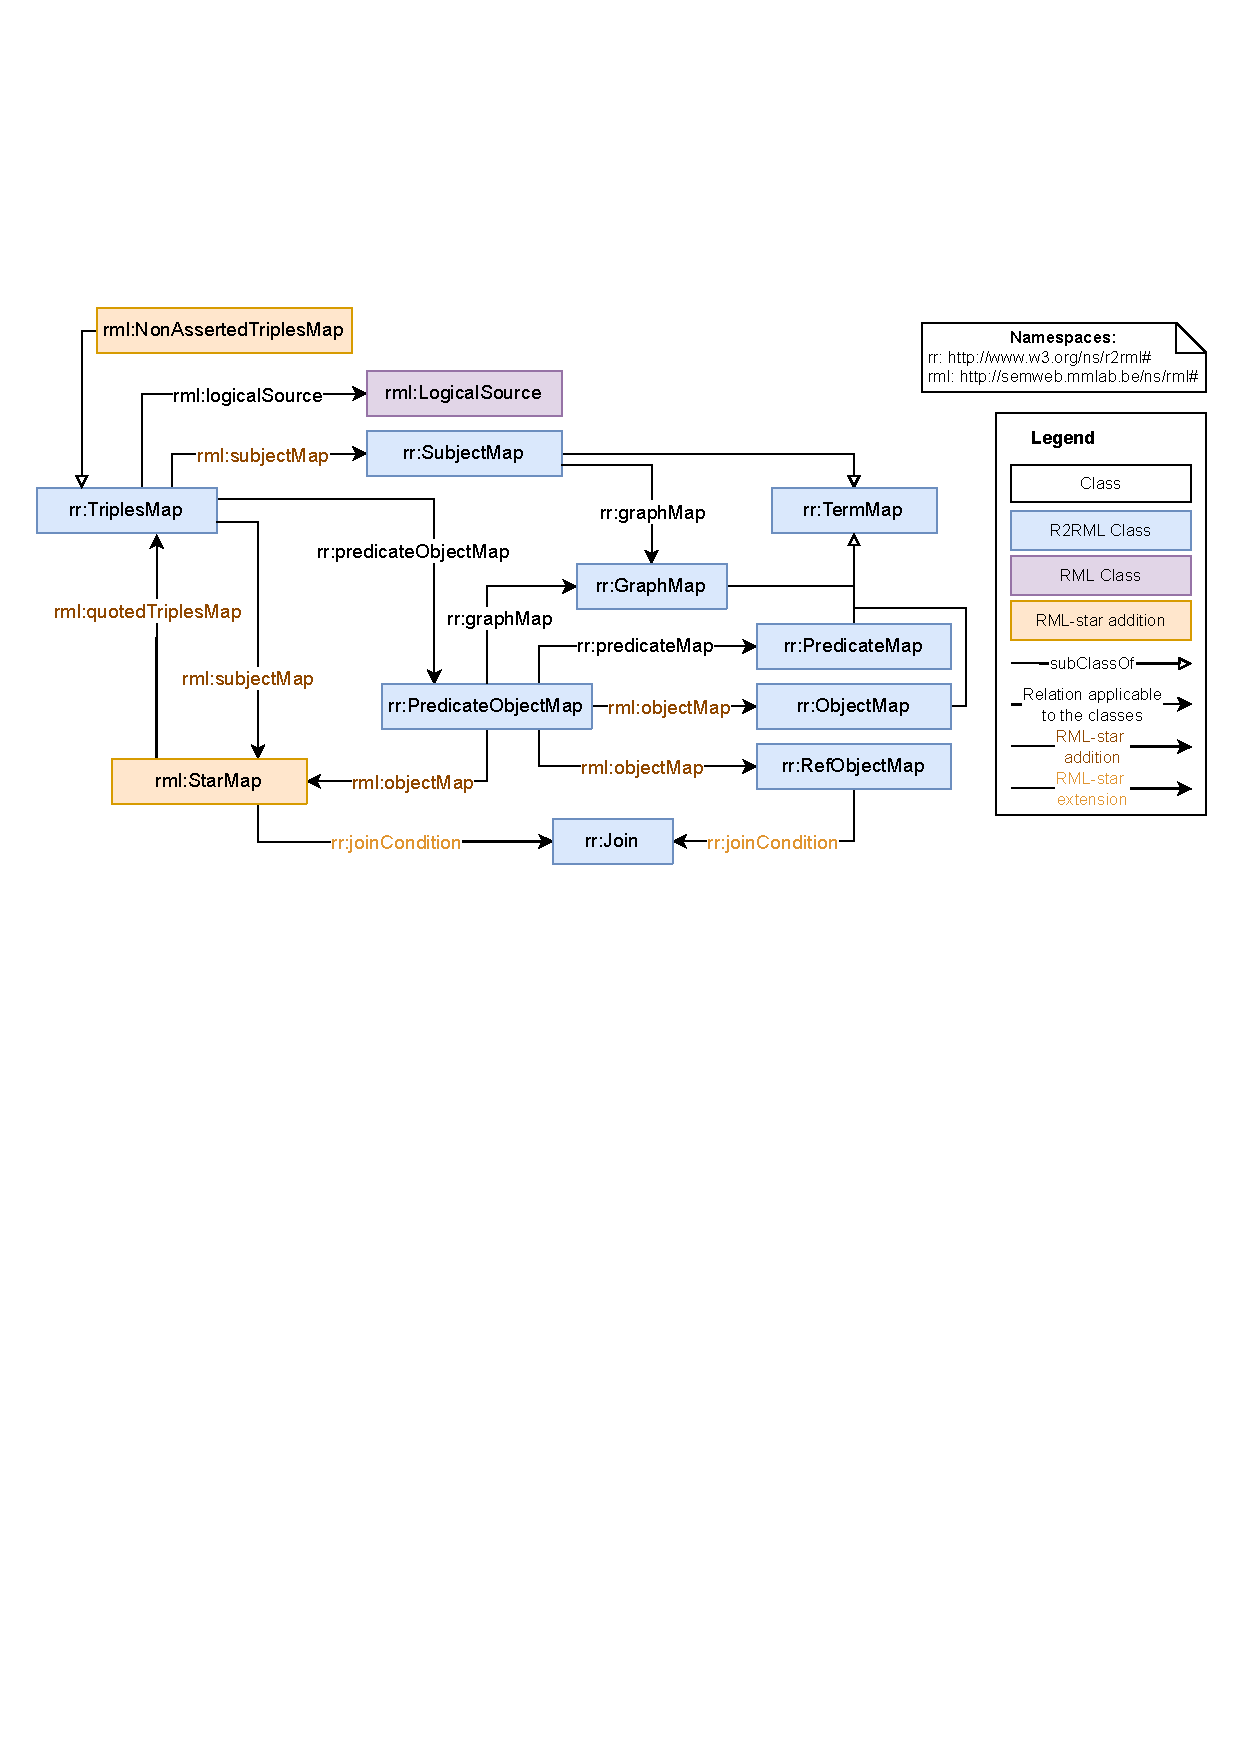
\includegraphics[width=1\linewidth]{figures/rml-star_diagram.pdf}
\caption{The \mbox{RML-star} extension (represented using the Chowlk notation~(\cite{feria2022chowlk})) with additions and modifications over the RML ontology.}
\label{fig:rml-star}
\end{figure*}

\begin{minipage}{\linewidth}
\centering
\begin{captionedlisting}{lst:chp4_rml-star}{Example RML-star mapping that transforms data in \cref{lst:chp4_csv_star}.}
\centering
\begin{multicols}{2}
{\begin{lstlisting}[numbers=left,basicstyle=\ttfamily\small,label={list:example1},columns=flexible,]
<#jumpTM> 
 a rml:NonAssertedTriplesMap ;
 rml:logicalSource :marks ;
 rml:subjectMap [ 
  rr:template ":{PERSON}" ] ;
 rr:predicateObjectMap [ 
  rr:predicate :jumps ;
  rml:objectMap [
   rml:reference "MARK" ] ] .
<#dateTM> 
 a rr:TriplesMap ;
 rml:logicalSource :marks ;
 rml:subjectMap [ 
  rml:quotedTriplesMap <#jumpTM>];
 rr:predicateObjectMap [ 
  rr:predicate :date ;
  rml:objectMap [
   rml:reference "DATE" ] ] .
\end{lstlisting}}

\end{multicols}
\end{captionedlisting}
\end{minipage}

\noindent\hspace{0.1\linewidth}\begin{minipage}{\linewidth}
\begin{captionedlisting}{lst:chp4_res-rml-star}{RDF-star triples generated by the mapping in \cref{lst:chp4_rml-star}.}
\centering
\begin{tabular}{c}
\hspace{2em}
{\begin{lstlisting}[basicstyle=\ttfamily\small,label={list:example1},columns=flexible]
<< :Angelica :jumps "4.80" >> :date "2022-03-21" .
<< :Katerina :jumps "4.85" >> :date "2022-03-19" .
\end{lstlisting}}
\end{tabular}
\end{captionedlisting}
\end{minipage}







\subsection{Validation}
\label{sec:chp4_validation}

We present the development of the RML star test-cases (\cref{sec:chp4_star_testcases}), that enables new implementations to check their conformance to RML-star; and create RML-star mappings for two real-world use cases (in \cref{sec:chp4_star_usecases}): software metadata extraction~(\cite{kelley2021framework} (SoMEF)) and biomedical research literature~(\cite{SemMedDB}) (SemMedDB). We use for both cases \mbox{Morph-KGC$^{star}$}, an implementation of RML-star.




\subsubsection{RML-star Test Cases}
\label{sec:chp4_star_testcases}

Test cases are commonly used %in standardization processes 
to evaluate the conformance of an engine with respect to a language specification (e.g., RML test cases~(\cite{heyvaert2019conformance})). 
A set of \mbox{RDF-star} test cases was proposed
covering the syntax of various of its serializations\footnote{\url{https://w3c.github.io/rdf-star/tests/}}.
We adapted these test cases to create the RML-star test cases and evaluate the conformance of \mbox{Morph-KGC$^{star}$}
with respect to \mbox{RML-star}.

To create a representative set of test cases for \mbox{RML-star}, we selected the N-Triples-star syntax tests\footnote{\url{https://w3c.github.io/rdf-star/tests/nt/syntax}}.  %;and follow a reverse engineering process. 
For each \mbox{RDF-star} test case, we created two associated \mbox{RML-star} test cases that generate the original \mbox{RDF-star} dataset: one test case with a single input data source (i.e., the mapping does not include joins) and another with two input data sources (i.e., the mapping includes joins among triple maps).
For each test case, we manually created the input source(s) in the CSV format and the corresponding \mbox{RML-star} mapping rules to generate the output \mbox{RDF-star} datasets.
Following this approach, we obtained 16 \mbox{RML-star} test cases.
The test cases are openly available at the W3C Community Group on Knowledge Graph Construction~(\footnote{\url{https://github.com/kg-construct/rml-star-test-cases}}),
and can be reused by any engine to test its conformance with respect to \mbox{RML-star}.


\subsubsection{Use Cases}
\label{sec:chp4_star_usecases}

We create RML-star mappings for in two real-world use cases. 
The first generates \mbox{RDF-star} graphs from scientific software documentation, 
and the second annotates statements extracted from biomedical research publications. 
For both use cases, we use the tool \mbox{Morph-KGC$^{star}$}.









%In order to ensure that these results in terms of time are representative, we run each mapping three times and calculate the average time.

%In both use cases we report the time on generating the RDF-star datasets. 




%In summary, our test and use cases show that \mbox{Morph-KGC$^{star}$} generates valid RDF triples and does not add an overhead in the generation time of reified triples. However, a more thorough analysis (out of the scope of this paper) is required to describe the behaviour of each mapping approach.

\noindent\textbf{\textit{Scientific Software Metadata Extraction.}}
Scientific software has become a crucial asset to deliver and reproduce the results described in research publications~(\cite{chue_hong_fair_2021}). However, scientific software is often time consuming to understand and reuse due to incomplete and heterogeneous documentation, available only in a human-readable manner.
The Software Metadata Extraction Framework (SoMEF)~(\cite{somef}) proposes an approach to automatically extract relevant metadata (description, installation instructions, citation, etc.) from code repositories and their documentation. SoMEF includes different text extraction techniques (e.g., supervised classification, regular expressions, etc.) that yield results with different confidence values.
For example, \cref{lst:JSONsnippet} shows a JSON snippet with the description that SoMEF obtained from a software repository (Widoco) using the GitHub API.
The confidence in this case is high as the extracted description was manually curated by the creators of the code repository.
SoMEF extracts more than 30 different metadata fields about 
software, its source code, its released versions, and their corresponding authors. For transforming the output of SoMEF into RDF-star, we used a total of 35 triples maps to annotate software metadata fields and an additional triples map to annotate source code descriptions. All reified triples follow the same structure (Listings \ref{lst:JSONsnippet} \& \ref{lst:TTLsnippet}), i.e. the standard RDF triple contains the excerpt of the extracted feature, and it is annotated
with the \emph{technique} used and the \emph{confidence} value. 
The complete mapping and all input examples and results are available online\footnote{\url{https://github.com/oeg-upm/rdf-star-generation}}.
 
\noindent\hspace{0.1\linewidth}\begin{minipage}{0.8\linewidth}
\begin{captionedlisting}{lst:JSONsnippet}{JSON snippet showing the description metadata field extracted by SoMEF on a code repository using the GitHub API as extraction technique.}
\centering
\hspace{3em}
{
\begin{lstlisting}[basicstyle=\ttfamily\small,label={list:example1},columns=flexible]
"codeRepository": "https://github.com/oeg-upm/Widoco",
"description": [ 
  {
    "confidence": [
      1.0
    ],
    "excerpt": "Wizard for documenting ontologies. WIDOCO is ...",
    "technique": "GitHub API"
  }
]  
\end{lstlisting}
}
\end{captionedlisting}
\end{minipage}

Capturing the technique used and the confidence obtained for each extracted metadata field is key for obtaining an accurate representation of the result. Hence, the \mbox{RDF-star} representation corresponding to the JSON in \cref{lst:JSONsnippet} includes this information, as depicted in \cref{lst:TTLsnippet}.

%\begin{minipage}{0.9\linewidth}
%\begin{captionedlisting}{lst:TTLsnippet}{N-Triples-star snippet showing the results generated for the %description field shown in \cref{lst:JSONsnippet}. Each asserted triple is annotated with its %corresponding confidence and technique.}
%\centering
%\begin{tabular}{c}
%\hspace{1.4em}
%{
%\begin{lstlisting}[numbers=left]
%<< <https://example.org/oeg-upm/Widoco> <https://w3id.org/okn/o/sd#description> 
%    "Wizard for documenting ontologies. WIDOCO is ..." >> 
%        <https://www.w3id.org/okn/o/em#technique> "GitHub API" .
%<< <https://example.org/oeg-upm/Widoco> <https://w3id.org/okn/o/sd#description> 
%    "Wizard for documenting ontologies. WIDOCO is ..." >> 
%        <https://www.w3id.org/okn/o/em#confidence> "1.0" .
%<https://example.org/oeg-upm/Widoco> <https://w3id.org/okn/o/sd#description> 
%    "Wizard for documenting ontologies. WIDOCO is ..." .
%\end{lstlisting}
%}
%\end{tabular}
%\end{captionedlisting}
%\end{minipage}        


\begin{captionedlisting}{lst:TTLsnippet}{RDF-star triples snippet showing the results generated for the description field in \cref{lst:JSONsnippet}. Each asserted triple is annotated with its corresponding confidence and technique.}
\centering
{
\begin{lstlisting}[basicstyle=\ttfamily\small,label={list:example1},columns=flexible]
ex:oeg-upm/Widoco :description "Wizard for documenting ontologies. WIDOCO is ..." .
<<ex:oeg-upm/Widoco :description "Wizard for documenting ontologies. WIDOCO is ...">> 
    :technique "GitHub API" .
<<ex:oeg-upm/Widoco :description "Wizard for documenting ontologies. WIDOCO is ...">> 
    :confidence "1.0" .
\end{lstlisting}
}
\end{captionedlisting}


%For example, for \cref{lst:JSONsnippet}, the excerpt of the software's description ("Wizard for documenting ontologies. WIDOCO is ...") was extracted with the technique "GitHub API" with a confidence of 1.0. 
% talk about the execution
%The reified triples are used for describing the software, that uses


\noindent\textbf{\textit{Biomedical Research Literature.}} 
SemMedDB~(\cite{SemMedDB}), the Semantic MEDLINE Database, is a repository 
that contains information on extracted biomedical entities 
and predications (subject-predicate-object triples) 
from biomedical texts (titles and abstracts from PubMed citations). 
%consists of a set of triples and annotations automatically extracted from PubMed titles, abstracts, and citations. 
%a set of data sources with automatic semantic annotations from titles and abstracts of citations available in PubMed.
The tables comprising SemMedDB are available for download as a relational database or CSV files\footnote{ \url{https://lhncbc.nlm.nih.gov/ii/tools/SemRep_SemMedDB_SKR/SemMedDB_download.html}}.
We downloaded the MySQL files for (1)~predication predictions (PREDICATION and PREDICATION\_AUX tables), containing more than 117 million annotations; and (2)~entity predictions (ENTITY table), which include more than 410 million annotations.
Listings \ref{lst:chp4_semmeddb_entity}, \ref{lst:chp4_semmeddb_pred} and \ref{lst:chp4_semmeddb_predaux} illustrate the columns used from the tables with synthetic data. 
For predications, only data for subjects is shown; the missing columns regarding objects follow the same structure as subjects.
%This data contains information on predicted entities and predicted subject-predicate-object predications.
Subjects and objects, from predications, and entities are assigned a semantic type 
(that categorizes the extracted concept in the biomedical domain) annotated with a confidence score. 
In addition, the extraction of subjects and objects is assigned a timestamp on when it took place. 
Thus, the score and timestamp represent metadata about other statements.
We created an RML-star mapping with 5 triples maps quoting triples:
3 of them are used to annotate the assignation of semantic types to entities, subjects, and objects with confidence scores;
the remaining 2 provide the timestamps for the extraction of subjects and objects. 

\begin{minipage}{0.38\linewidth}
\begin{captionedlisting}{lst:chp4_semmeddb_entity}{ENTITY table snippet.}
\centering
\begin{tabular}{c}
\hspace{-1em}
{
\begin{lstlisting}[basicstyle=\ttfamily\small,label={list:example1},columns=flexible]
ENTITY_ID , SEMTYPE , SCORE
12345     , orga    , 790
\end{lstlisting}
}
\end{tabular}
\end{captionedlisting}
\end{minipage}
\,\,\,\,\hfill
\begin{minipage}{0.6\linewidth}
\begin{captionedlisting}{lst:chp4_semmeddb_pred}{PREDICATION table snippet.}
\centering
\begin{tabular}{c}
\hspace{-1em}
{
\begin{lstlisting}[basicstyle=\ttfamily\small,label={list:example1},columns=flexible]
PREDICATION_ID , SUBJECT_SEMTYPE , SUBJECT_NAME
13579          , Semtype         , SubjName
\end{lstlisting}
}
\end{tabular}
\end{captionedlisting}
\end{minipage}

\noindent\hspace{0.23\linewidth}\begin{minipage}{0.8\linewidth}
\begin{captionedlisting}{lst:chp4_semmeddb_predaux}{PREDICATION\_AUX table snippet.}
\centering
\begin{tabular}{c}
\hspace{-7em}
{
\begin{lstlisting}[basicstyle=\ttfamily\small,label={list:example1},columns=flexible]
PREDICATION_AUX_ID, PREDICATION_ID, SUBJECT_SCORE, TIMESTAMP
67890             , 13579         , 800          , 1651740766
\end{lstlisting}
}
\end{tabular}
\end{captionedlisting}
\end{minipage}

\noindent\hspace{0.1\linewidth}\begin{minipage}{0.78\linewidth}
\begin{captionedlisting}{lst:chp4_semmeddb_triples}{RDF-star triples generated from data in Listings \ref{lst:chp4_semmeddb_entity}, \ref{lst:chp4_semmeddb_pred} and \ref{lst:chp4_semmeddb_predaux}.}
\centering
\begin{tabular}{c}
\hspace{-1.5em}
{
\begin{lstlisting}[basicstyle=\ttfamily\small,label={list:example1},columns=flexible]
<<ex:12345 sem:semanticType "orga">> sem:score "790" .
<<ex:13579 sem:subject ex:SubjName>> sem:timestamp "1651740766" .
<<ex:SubjName sem:semanticType "Semtype">> sem:score "800" .
\end{lstlisting}
}
\end{tabular}
\end{captionedlisting}
\end{minipage}


\section{Conclusions}

This chapter addresses the fist objective of this thesis \textit{O1:To analyze the needs for declarative knowledge graph construction from heterogeneous data sources, in order to facilitate the support of advances in existing mapping languages to address the most relevant ones.} 
To reach this objective, we first performed an in-depth analysis of the features of the current mapping languages: from the description of input data sources, to the diverse features for triple generation. This comprises the first contribution of \textit{O1, C1: Design of a comparison framework analysing the state of the art mapping languages.}
This analysis and the challenges proposed by the Knowledge Graph Construction W3C Community Group are gathered as requirements for a mapping language to be able to address the complexity of use cases for KG construction. 

Then, we presented the Conceptual Mapping, an ontology that, based on the abovementioned requirements, gathers the expressiveness of current mapping languages. This ontology was developed following the LOT methodology, it is evaluated accordingly and made available under a W3ID. 
This comprises the second contribution ob objective O1, \textit{C2: Identify, define and implement the requirements for knowledge graph construction from heterogeneous data sources.}

Finally, we show that mapping languages evolve as KG technologies advance, in this case with the adoption of RDF-star. To that purpose, we extend one of the most used mapping languages, RML, to create RDF-star graphs, RML-star. Accordingly, we add an extension to the Conceptual Mapping to include this new feature. This comprises the third contribution of objective O1, \textit{C3 Development of new features for the RML mapping language.}

Our ambition with these contributions is to enhance the understanding of the capabilities of mapping languages and what they need to implement in order to cover the necessities for constructing knowledge graphs, and at the same time be able to evolve as the technologies progress.